\documentclass[11pt,a4paper,english,greek,twoside]{dblab-thesis}
\usepackage{epsfig}
%\usepackage[english,greek]{babel}
%\usepackage[T1]{fontenc}
%\usepackage[iso-8859-7]{inputenc}
%\usepackage{graphicx}
%\DeclareGraphicsRule{.tif}{bmp}{}{}
%\usepackage[explicit]{titlesec}
\usepackage{indentfirst}
\usepackage{verbatim}
\usepackage{amsmath}
\usepackage{subcaption}
\usepackage{amsthm}
\usepackage{amssymb}
\usepackage{epstopdf}
\usepackage{latexsym}
\usepackage{index}
\usepackage{datetime}
\usepackage{textcomp}
\usepackage{graphicx}
\usepackage{url}
\usepackage{array}
\usepackage{algorithm}
\usepackage{algorithmic}
\usepackage{babel}
\usepackage{afterpage}
\usepackage{caption}
\usepackage{bbm}
\usepackage{multirow}
\usepackage{longtable}
%\usepackage{makeidx}
%\bibliographystyle{alpha}
%\bibliographystyle{abbrv}
\bibliographystyle{plain}

\newindex{default}{idx}{ind}{Ευρετήριο όρων}
\newindex{en}{edx}{end}{Ευρετήριο αγγλικών όρων}
%\makeindex


% Page definitions
%\setlength{\textheight}{23cm} \setlength{\textwidth}{15.5cm}
%\setlength{\oddsidemargin}{0.2cm}
%\setlength{\evensidemargin}{0.2cm} \setlength{\topmargin}{-1.2cm}
%\setlength{\headsep}{1.5cm}

% 1.5 spacing
\renewcommand{\baselinestretch}{1.2}

\newcommand\blankpage{%
    \null
    \thispagestyle{empty}%
    \addtocounter{page}{-1}%
    \newpage}
% latin text (and greek text)
%\newcommand{\prg}[1]{\textlatin{\texttt{#1}}}
\newcommand{\tl}[1]{\textlatin{#1}}
\newcommand{\tg}[1]{\textgreek{#1}}

% typeset short english phrases
\newcommand{\en}[1]{\foreignlanguage{english}{#1}}

% typeset source code
\newcommand{\src}[1]{{\tt\en{#1}}}



% typeset a backslash
\newcommand{\bkslash}{\en{\symbol{92}}}

%typeset infx(a) supx(a) etc
%\newcommand{\infx}[1]{inf_x({#1})}
%\newcommand{\infy}[1]{inf_y({#1})}
%\newcommand{\supx}[1]{sup_x({#1})}
%\newcommand{\supy}[1]{sup_y({#1})}
%\newcommand{\dlt}{\delta}
%\newcommand{\most}{${\cal M}ost$}
%\newcommand{\br}{${\cal B}r$}
\newcommand*\Hide{%
\titleformat{\chapter}[display]
  {}{}{0pt}{\Huge}
\titleformat{\part}
  {}{}{0pt}{}
}
\newtheorem{definition}{Ορισμός}
\newtheorem{proposition}{Πρόταση}
\newtheorem{theorem}{Θεώρημα}
\newtheorem{corollary}{Συμπέρασμα}
\newtheorem{lemma}{Λήμμα}
\newtheorem{example}{Παράδειγμα}
\newtheorem{remark}{Σημείωση}
\newtheorem{notation}{Συμβολισμός}
\newtheorem{law}{Νόμος}
\renewcommand{\thedefinition}{\arabic{chapter}.\arabic{definition}}
\renewcommand{\theproposition}{\arabic{chapter}.\arabic{proposition}}
\renewcommand{\thetheorem}{\arabic{chapter}.\arabic{theorem}}
\renewcommand{\thecorollary}{\arabic{chapter}.\arabic{corollary}}
\renewcommand{\thelemma}{\arabic{chapter}.\arabic{lemma}}
\renewcommand{\theexample}{\arabic{chapter}.\arabic{example}}
\newcommand{\set}[1]{\left\{#1\right\}}
\newcommand{\To}{\Longrightarrow}
\newcommand{\xml}{\en{XML}}


\selectlanguage{greek}
\hyphenation{τμή-μα Επο-μέ-νως}

\title{Βελτίωση ακρίβειας στατιστικών μεθόδων πρόβλεψης σε χρονοσειρές μικρού ιστορικού με χρήση τεχνικών συσταδοποίησης εποχιακών δεικτών συναφών δεδομένων}
\author{Ευάγγελος Νταβέλης}
\supervisor{Βασíλειος Ασημακóπουλος}
\TRnumber{ΕΣΒΓΔ-ΔΙΠΛ-2015-03}
\epitropiF{Ιωάννης Ψαρράς}
\epitropiS{Δημήτριος Ασκούνης}


\begin{document}
\selectlanguage{greek}
\maketitle

\frontmatter
\pagenumbering{roman}
\mainmatter
\begin{acknowledgements}

Θα ήθελα να ευχαριστήσω τον επιβλέποντα καθηγητή κ. Νικόλαο Χατζηαργυρίου για την ευκαιρία που μου έδωσε να εκπονήσω τη παρούσα διπλωματική και την υποστήριξή του σε όλη την πορεία της.

Επίσης, θα ήθελα να ευχαριστήσω  τους καθηγητές κ. Σταύρο Παπαθανασίου και κ. Παύλο Γεωργιλάκη για την τιμή που μου έκαναν να συμμετάσχουν στην επιτροπή εξέτασης της διπλωματικής.

Eυχαριστώ ιδιαίτερα τον υποψήφιο διδάκτορα Γιώργη Μεσσήνη για την καθοδήγηση, στήριξη και καθοριστική βοήθεια που μου παρείχε.

Τέλος, θα ήθελα να ευχαριστήσω την οικογένειά μου και τους φίλους μου που παρέχουν πάντοτε ένα χέρι βοήθειας σε ό,τι χρειαστώ.

\end{acknowledgements}


\begin{abstract}
Οι εταιρίες παροχής ηλεκτρισμού αντιμετωπίζουν το ολοένα και αυξανόμενο πρόβλημα της διείσδυσης μη τεχνικών απωλειών στις καταναλώσεις των πελατών τους. Το γεγονός αυτό πλήττει σημαντικά τις εταιρίες, μειώνοντας το εισόδημά τους και θέτει σε κίνδυνο τους ανειδίκευτους καταναλωτές που επεμβαίνουν στις υποδομές του παρόχου. Η προσέγγιση αυτού του προβλήματος έγινε με προσομοίωση ρευματοκλοπών σε ετήσιες χρονοσειρές καταναλωτών και δοκιμάστηκαν πληθώρα αλγορίθμων επιβλεπόμενης, μη επιβλεπόμενης και ημι-επιβλεπόμενης μηχανικής μάθησης για την ανίχνευση των καταναλωτών με διείσδυση μη τεχνικών απωλειών. Τα αποτελέσματα αναδεικνύουν τις δυνατότητες των συστημάτων μη επιβλεπόμενης και ημι-επιβλεπόμενης μάθησης σε σχέση με τη δεδομένη επιτυχία των αλγορίθμων επιβλεπόμενης μάθησης. Τα συστήματα που δημιουργήθηκαν έχουν ικανοποιητική απόδοση που δεν αποκλίνει σημαντικά από τους αλγορίθμους αναφοράς της επιβλεπόμενης μάθησης. Καθίσταται λοιπόν σαφές πως η ανίχνευση μη τεχνικών απωλειών είναι εφικτή με συστήματα μηχανικής μάθησης.

\begin{keywords}
  Μη τεχνικές απώλειες, Ρευματοκλοπές, Χρονοσειρές, Μηχανική μάθηση, Επιβλεπόμενοι αλγόριθμοι, Μη επιβλεπόμενοι αλγόριθμοι, Ημι-επιβλεπόμενοι αλγόριθμοι.
 
\end{keywords}

\end{abstract}



\begin{abstracteng}
\tl{Power companies face the problem of increasing intrusion of non-technical losses on consumptions of their clients. That fact hurts significantly power companies by reducing their economical growth and sets on danger unskilled consumers who intervene with the power infastracture. This problem was approached by simulating frauds on yearly timeseries and by testing  many different algorithms of supervised, unsupervised and semi-supervised  machine learning in order to detect consumers with non-technical loss intrusion. The results show the potencial of the unsupervised and semi-supervised learning in relation with the given success of supervised algorithms. The created systems have satisfactory performance which does not diverge significantly from the reference algorithms of supervised learning. Concluding the detection of non-technical losses is achievable with machine learning systems.}
\begin{keywordseng}
  \tl{Non-technical losses, power fraud, Timeseries, Machine learning, Supervised algorithms, Unsupervised algorithms, Semi-supervised algorithms.}
\end{keywordseng}

\end{abstracteng}

\tableofcontents
\listoffigures
\listoftables
\chapter{Εισαγωγή}
\label{chap1}

Στις κλασικές στατιστικές μεθόδους πρόβλεψης χρονοσειρών η συνηθισμένη διαδικασία ακολουθεί μια συγκεκριμένη διαδικασία βημάτων. Αρχικά, προετοιμάζουμε τη χρονοσειρά για ανάλυση. Έπειτα, την αναλύουμε στις τέσσερις της συνιστώσες: την τάση, την εποχιακότητα, την κυκλικότητα και την τυχαιότητα. Η πρόβλεψη γίνεται στην αποεποχικοποιημένη χρονοσειρά και μετά ενσωματώνεται σε αυτή το στοιχείο της εποχιακότητας.

Όμως, τα εργαλεία για αποσύνθεση της χρονοσειράς που έχουμε στη διάθεσή μας απαιτούν η χρονοσειρά να έχει τουλάχιστον ένα πλήθος παρατηρήσεων. Σε αντίθετη περίπτωση, η χρονοσειρά προβλέπεται σαν να μην χαρακτηρίζεται από εποχιακή συμπεριφορά. Το πρόβλημα προκύπτει λοιπόν στην αδυναμία να συνυπολογίσουμε την επιρροή της εποχιακότητας στην πρόβλεψη χρονοσειρών με μικρό ιστορικό.

Παράλληλα, ζούμε σε μια εποχή που την χαρακτηρίζει αφθονία δεδομένων. Έτσι συναντάμε όλο και περισσότερο χρονοσειρές που είναι μέρος ενός ευρύτερου συνόλου που περιγράφει παρόμοια μεγέθη.


\section{Αντικείμενο της διπλωματικής}

Στη παρούσα διπλωματική θα προσπαθήσουμε να χρησιμοποιήσουμε τη πληροφορία που μας δίνεται από ένα μεγάλο σύνολο δεδομένων για να προβλέψουμε με μεγαλύτερη ακρίβεια μικρές χρονοσειρές.

Θα χωρίσουμε, λοιπόν, τις χρονοσειρές σε μικρές και μεγάλες, δηλαδή με επαρκές ιστορικό για αποεποχικοποίηση. Στις μεγάλες χρονοσειρές θα χρησιμοποιήσουμε τις γνωστές μεθόδους αποσύνθεσης για να παραγάγουμε τους δείκτες εποχιακότητας για κάθε μία από αυτές. Στις μικρές, θα υπολογίσουμε ένα σύνολο δεικτών ψευδο-εποχιακότητας.

Χρησιμοποιώντας τεχνικές συσταδοποίησης στη πρώτη ομάδα των χρονοσειρών θα ελέγξουμε αν υπάρχουν πράγματι μοτίβα εποχιακότητας που χαρακτηρίζουν υποσύνολα των δεδομένων και θα τα εντοπίσουμε. Μετά θα εξετάσουμε αν οι μικρές χρονοσειρές δύνανται να καταταχθούν σε κάποια από τις συστάδες που υπολογίσαμε βάσει των δεικτών ψευδο-εποχιακότητας τους.

Στη συνέχεια, θα προεκτείνουμε τις μικρές χρονοσειρές που βρήκαμε να ανήκουν σε κάποια συστάδα στο μέλλον με δύο τρόπους. Πρώτα, θα τις προβλέψουμε όπως γίνεται συνήθως. Έπειτα, θα τις αποεποχικοποιήσουμε βάσει της μέσης εποχιακότητας των μεγάλων χρονοσειρών που ανήκουν στην ίδια συστάδα με αυτές, θα τις προβλέψουμε και θα τις επαναεποχικοποιήσουμε.

Τελικά θα εκτιμήσουμε αν η ακρίβεια της προτεινόμενης μεθόδου είναι μεγαλύτερη από τη κλασική προσέγγιση.


\subsection{Συνεισφορά}

Η συνεισφορά της διπλωματικής συνοψίζεται ως εξής:

\begin{enumerate}
\item Μελετήθηκε ένα σύνολο χρονοσειρών που περιγράφει το επίπεδο φυσικού αερίου σε δεξαμενές
\item Έγινε ανάλυση τους και μετατράπηκαν σε μορφή για μεσοπρόθεσμη πρόβλεψη
\item Υπολογίστηκαν οι ομάδες συνάφειας των μοτίβων εποχιακότητας
\item Βάσει αυτών αποεποχικοποιήσαμε χρονοσειρές μικρού ιστορικού
\item Μετρήσαμε ότι η ακρίβεια πρόβλεψης βελτιώνεται με την προτεινόμενη μέθοδο αποεποχικοποίησης
\end{enumerate}


\section{Οργάνωση του τόμου}

Ακολουθεί εκτενής περίληψη της διπλωματικής στο Κεφάλαιο \ref{chapabst}. Στο Κεφάλαιο \ref{chap2} θα περιγράψουμε τι είναι μια χρονοσειρά, τα δομικά της στοιχεία και θα δωθεί ιδιαίτερη προσοχή στην εποχιακή της συμπεριφορά, πώς μπορούμε να την απομονώσουμε ή να την ενσωματώσουμε στο μοντέλο της πρόβλεψης. Η μεθοδολογία που ακολουθείται για τη πρόβλεψη μιας χρονοσειράς, δηλαδή η προετοιμασία της, η προέκτασή της στο μέλλον και τέλος η αξιολόγησή ακρίβειας αναλύονται στο Κεφάλαιο \ref{chap3}. Στο Κεφάλαιο \ref{chap4} παραθέτουμε αναλυτικά τα βήματα που ακολουθούμε για να αντιμετωπίσουμε το πρόβλημα των εποχιακών μικρών χρονοσειρών. Συγκεκριμένα, πώς εφαρμόζονται αυτά τα βήματα στο υπό εξέταση σύνολο δεδομένων φαίνεται στο Κεφάλαιο \ref{chap5}.  Στο Κεφάλαιο \ref{chap8} συνοψίζουμε τα αποτελέσματα και συζητάμε μελλοντικές επεκτάσεις.
Τέλος, στο παράρτημα, ακολουθούν οι γλώσσες προγραμματισμού, οι βιβλιοθήκες και τα περιβάλλοντα ανάπτυξης που χρησιμοποιήθηκαν για την υλοποίηση του πειράματος της διπλωματικής και η παράθεση των λεπτομερών αποτελεσμάτων μέτρησης της ακρίβειας.


\chapter{Εκτενής Περίληψη}
\label{chapabst}

Χρονοσειρά ονομάζουμε ένα σύνολο παρατηρήσεων που περιγράφουν την εξέλιξη της συμπεριφοράς ενός μεγέθους στο χρόνο. Θεωρούμε, μάλιστα, ότι αυτές οι παρατηρήσεις δεν είναι ανεξάρτητες μεταξύ τους χωρίς βέβαια αυτό να υπονοεί μια ντετερμινιστική σύνδεση μεταξύ αυτών. 

Οι χρονοσειρές μπορούν να αναλυθούν σε τέσσερις χαρακτηριστικές υποσειρές. Την τάση, που περιγράφει πως μεταβάλλεται χρονικά το επίπεδο της χρονοσειράς. Τη κυκλικότητα που μετράει την κατά περιόδους μεταβολή της χρονοσειράς που οφείλεται σε εξωγενείς συνθήκες. Την εποχιακότητα που αποτελεί το μοτίβο διακύμανσης που παρουσιάζει η χρονοσειρά και επαναλαμβάνεται ανά σταθερές χρονικές περιόδους. Ο αστάθμητος παράγοντας της τύχης μιας χρονοσειράς καλείται τυχαιότητα.

Υπάρχει ένα σύνολο μεθόδων που μας επιτρέπει να αποσυνθέσουμε τη χρονοσειρά στα επιμέρους της στοιχεία. Εν γένει αντιμετωπίζουμε τη χρονοσειρά είτε ως άθροισμα των συνθετικών της μονάδων, είτε ως γινόμενο. Η πρώτη προσέγγιση είναι η προσθετική, ενώ η δεύτερη η πολλαπλασιαστική. Χρησιμοποιώντας το στατιστικό εργαλείο των κινητών μέσων όρων μπορούμε να εφαρμόσουμε τη κλασική μέθοδο αποσύνθεσης είτε με την προσθετική είτε με την πολλαπλασιαστική προσέγγιση. Συμπληρωματικά, για να εξασφαλίσουμε υψηλή ακρίβεια στον υπολογισμό των δεικτών εποχιακότητας μπορούμε να ενσωματώσουμε στη διαδικασία υπολογισμού της εποχιακότητας της χρονοσειράς μία μέθοδο συρρίκνωσης συντελεστών όπως είναι η μέθοδος \en{James-Stein} ή η μέθοδος \en{Lemon-Krutchkoff}.

Μία άλλη μέθοδος αποσύνθεσης είναι η μέθοδος \en{STL}. Αποτελεί ουσιαστικά μία διαδικασία φιλτραρίσματος της χρονοσειράς που μας επιτρέπει να την αποδομήσουμε σε τρία βασικά χαρακτηριστικά: την τάση, την εποχιακότητα και τα εναπομείνοντα στοιχεία. Η διαδικασία βασίζεται στη μέθοδο \en{Loess}.

Εκτός των παραπάνω μεθόδων που είναι ανεξάρτητες της διαδικασίας της πρόβλεψης, αν και αποτελεί συνήθως τον τελικό στόχο, υπάρχουν μοντέλα που ενσωματώνουν την εποχιακή ανάλυση. Ένα τέτοιο παράδειγμα είναι η μέθοδος \en{Holt-Winters} που στηρίχθηκε στη μέθοδο εκθετικής εξομάλυνσης για χρονοσειρές γραμμικής τάσης και είναι ικανή να διαχειριστεί και την εποχιακότητα. Επίσης, τα ολοκληρωμένα αυτοπαλινδρομικά μοντέλα κινητών μέσω όρων \en{(ARIMA)} δύνανται να μοντελοποιήσουν ένα μεγάλο εύρος εποχιακών δεδομένων.

Γενικά η διαδικασία της πρόβλεψης είναι μια πολυβηματική διαδικασία που αποσκοπεί στη χρήση της γνώσης των παρελθοντικών παρατηρήσεων μιας χρονοσειράς για να εκτιμήσει πως αυτή θα εξελιχθεί στο μέλλον.

Αρχικά, πρέπει η χρονοσειρά να έρθει σε κατάλληλη μορφή για να μπορέσουμε να εφαρμόσουμε τις στατιστικές μεθόδους που την προεκτείνουν στο μέλλον. Έτσι, το πρώτο βήμα είναι να αναπαραστήσουμε γραφικά τα δεδομένα έτσι ώστε να αποκτήσουμε μια εποπτεία στα ποιοτικά της χαρακτηριστικά. Βάσει αυτών και της γνώσης που έχουμε εν γένει για τα δεδομένα, καλούμαστε στη συνέχεια να διαχειριστούμε τις ιδιομορφίες της χρονοσειράς. Αυτές μπορεί να είναι μη ιδανική δειγματοληψία, κενές τιμές ή μηδενικές. Επίσης, πολλές φορές η χρονοσειρά χρήζει ημερολογιακών προσαρμογών αφότου οι παρατηρήσεις της μπορούν να επηρεάζονται από τις ημέρες ανθρώπινης εργασίας και συνεπώς από τα σαββατοκύριακα ή και τις αργίες. 

Αφότου τα δεδομένα έχουν έρθει σε κατάλληλη μορφή και μπορούμε να τα αποσυνθέσουμε όπως περιγράψαμε προηγουμένως, χρειάζεται να τα προεκτείνουμε στο μέλλον. Μία πρώτη προσέγγιση είναι να θεωρήσουμε ότι κάθε μελλοντική στιγμή είναι ταυτόσημη με αυτή που προηγείται. Αυτή προσέγγιση περιγράφει τη μέθοδο \en{Naive} που συνήθως χρησιμοποιείται ως βάση σύγκρισης.

Η ανάλυση της παλινδρόμησης θεωρώντας τον χρόνο ανεξάρτητη μεταβλητή, αποτελεί μία άλλη μέθοδο προέκτασης της χρονοσειράς. Εν γένει αποσκοπεί στην εύρεση συσχετίσεων μεταξύ μιας εξαρτημένης μεταβλητής και μίας ή περισσότερων ανεξάρτητων μεταβλητών και γι' αυτό το λόγο εκτός από μοντέλο πρόβλεψης αυτή καθ' αυτή μπορεί να χρησιμοποιηθεί και ως υποβοήθημα για άλλες μεθόδους.

Τα μοντέλα εκθετικής εξομάλυνσης είναι απλά μοντέλα, εύκολα στη χρήση, με μικρές υπολογιστικές απαιτήσεις που έχουν την δυνατότητα να παράξουν ακριβείς προβλέψεις ακόμα και με σχετικά μικρό ιστορικό παρατηρήσεων. Τα συγκεκριμένα μοντέλα εξαρτώνται από τη μορφή της τάσης (Σταθερού επιπέδου, Γραμμικής, Εκθετικής ή Φθίνουσας τάσης) και από το πρότυπο εποχιακότητας (Χωρίς, Προσθετική, Πολλαπλασιαστική).

Η μέθοδος Θ βασίζεται στη μεταβολή των τοπικών καμπυλοτήτων μιας χρονοσειράς για να παράξει προβλέψεις. Η χρονοσειρά αναλύεται σε δύο ή περισσότερες γραμμές \en{Theta} και κάθε μία από αυτές προβλέπεται ξεχωριστά, είτε με το ίδιο είτε με διαφορετικό μοντέλο πρόβλεψης.

Αφότου έχουμε ολοκληρώσει τη διαδικασία της πρόβλεψης πρέπει να αξιολογήσουμε κατά πόσο το μοντέλο μας παρήγαγε ακριβείς προβλέψεις ή ποιο από τα μοντέλα που εφαρμόσαμε είναι καλύτερο. Για να το πετύχουμε αυτό χρησιμοποιούμε ένα σύνολο στατιστικών δεικτών αξιολόγησης της ακρίβειας. Αυτοί οι δείκτες μπορεί να εξαρτώνται από τη κλίμακα των δεδομένων ή να εκφράζονται από ποσοστιαία σφάλματα. Μπορούν να αντικατοπτρίζουν πραγματικά ή σχετικά μεγέθη, ή να είναι αποτέλεσμα κανονικοποίησης.

Στη παραπάνω διαδικασία, όμως, έχουμε πρόβλημα στη περίπτωση που η χρονοσειρά μας δεν διαθέτει αρκετά ιστορικά δεδομένα και συνεπώς δε μπορούμε να εξάγουμε το στοιχείο της εποχιακότητας. Η συνηθισμένη αντιμετώπιση είναι να θεωρήσουμε τη χρονοσειρά ως μη εποχιακή και να την προβλέψουμε ως τέτοια. Αλλά, έτσι ουσιαστικά δεν έχουμε απαλλάξει τη χρονοσειρά από τις εποχιακές της διακυμάνσεις και αυτές θα επηρεάσουν την ακρίβεια της πρόβλεψής μας. 

Ένας τρόπος να αντιμετωπίσουμε αυτό το ζήτημα είναι αν έχουμε ένα σύνολο χρονοσειρών που περιγράφουν συναφή μεγέθη. Έτσι, εκμαιεύουμε την πληροφορία για την εποχικότητα παρόμοιων χρονοσειρών και την χρησιμοποιούμε για να προβλέψουμε τις μικρότερες χρονοσειρές που φαίνεται να έχουν αντίστοιχη εποχιακή συμπεριφορά.

Για να το καταφέρουμε αυτό χρησιμοποιήθηκε η ακόλουθη μεθοδολογία. Αρχικά, φέρνουμε τα δεδομένα σε κατάλληλη μορφή για τις στατιστικές μεθόδους που θέλουμε να εφαρμόσουμε με τις συνηθισμένες τεχνικές διαχείρισης των ιδιομορφιών των χρονοσειρών και με χρήση της πληροφορίας που έχουμε για τα δεδομένα. Κατόπιν, χωρίζουμε τις χρονοσειρές σε δύο ομάδες: αυτές με επαρκή ιστορικά δεδομένα για να εξάγουμε την εποχιακή τους συμπεριφορά και τις υπόλοιπες.

Στη πρώτη κατηγορία, βρίσκουμε τους δείκτες εποχιακότητας με το κλασικό πολλαπλασιαστικό μοντέλο αποσύνθεσης. Στη συνέχεια, εφαρμόζουμε τον αλγόριθμο συσταδοποίησης \en{DBSCAN} στους υπολογισμένους δείκτες για να εντοπίσουμε αν υπάρχουν ομάδες με συνάφεια μεταξύ τους και να τις εντοπίσουμε. Για κάθε συστάδα υπολογίζουμε τους μέσους δείκτες εποχιακότητας.

Στη δεύτερη κατηγορία, υπολογίζουμε μία ψευδο-εποχιακότητα που θα χρησιμοποιήσουμε σαν κριτήριο συνάφειας για τις συστάδες που προέκυψαν προηγουμένως. Αν, λοιπόν, ένα διάνυσμα δεικτών έχει μικρότερη μέση τετραγωνική απόσταση από το μέσο όρο των εποχιακών δεικτών μίας συστάδας από την μέγιστη απόσταση που υπολογίζουμε από τις χρονοσειρές τις συστάδας και του μέσου όρου τους, τότε κατατάσσουμε την μικρή χρονοσειρά στην συστάδα.

Για τις μικρές χρονοσειρές που βρέθηκε να παρουσιάζουν κοντινή εποχιακή συμπεριφορά με κάποια συστάδα, χρησιμοποιούμε τους μέσους εποχιακούς δείκτες της συστάδας που ανήκουν ως την χαρακτηριστική τους εποχιακότητα. Κατόπιν, προβλέπουμε βάσει αυτής. Συγχρόνως, κάνουμε πρόβλεψη στα αρχικά δεδομένα και τελικώς συγκρίνουμε την ακρίβεια των δύο προσεγγίσεων σύμφωνα με το κανονικοποιημένο δείκτη μέσου απόλυτου σφάλματος.

Τα δεδομένα που έχουμε στη διάθεσή μας περιγράφουν τη στάθμη υγρού φυσικού αερίου σε ένα σύνολο δεξαμενών στη Γαλλία. Ο αρχικός σκοπός της ανάλυσης ήταν να εκτιμήσουμε πότε οι δεξαμενές αυτές θα αδειάσουν, έτσι ώστε να μπορεί η εταιρία διανομής να το αποτρέψει αλλά και να σχεδιάσει βέλτιστα τον ανεφοδιασμό τους. 

Για τη προετοιμασία τους ακολουθήσαμε τις εξής ενέργειες. Μετατρέψαμε τις αρνητικές και μηδενικές τιμές σε κενές τιμές. Μετατρέψαμε τα δεδομένα σε ημερήσια κρατώντας, στις περιπτώσεις πολλαπλών παρατηρήσεων εντός μίας ημέρας, τη μικρότερη από αυτές. Μετά συμπληρώσαμε τις κενές τιμές με τη μέθοδο της γραμμικής παρεμβολής βάσει του χρόνου.

Λόγω του ότι θέλουμε να προβλέψουμε πότε θα αδειάσει η κάθε δεξαμενή χρειαζόμαστε την χρονοσειρά ζήτησης. Γι' αυτό εφαρμόζοντας πρώτες διαφορές λαμβάνουμε την ημερήσια ζήτηση. Αφαιρέσαμε τους ανεφοδιασμούς και τους διαχειριστήκαμε ως κενές τιμές. Τέλος, έχοντας ως στόχο την μεσοπρόθεσμη ζήτηση, μετατρέψαμε τα δεδομένα μας σε μηνιαία, υπολογίζοντας τον μέσο όρο της ημερήσιας ζήτησης κάθε μήνα. 

Αφότου εφαρμόσαμε την αποεποχικοποίηση όπως περιγράφηκε προηγουμένως, εφαρμόσαμε τον αλγόριθμο \en{DBSCAN} που μας επέστρεψε μία συστάδα. Υπολογίσαμε τις μικρές χρονοσειρές που ανήκουν σε αυτή και εφαρμόσαμε τις δύο προσεγγίσεις για τη παραγωγή προβλέψεων. Για κάθε μία προσέγγιση, χρησιμοποιήσαμε έξι μοντέλα πρόβλεψης

Βρήκαμε ότι πράγματι βελτιώθηκε σημαντικά η ακρίβεια των προβλέψεών μας. Όλα τα μοντέλα πρόβλεψης είχαν μεγαλύτερη ακρίβεια, ενώ στο μεγαλύτερο ποσοστό των χρονοσειρών έδειξαν καλύτερα αποτελέσματα με την προτεινόμενη προσέγγιση. 



\chapter{Συγγενικές εργασίες}
\label{chap2}

\section{Εισαγωγή}

Εδώ γράφουμε σύντομα τις θεματικές περιοχές στις οποίες έχουμε ανακαλύψει συγγενικές εργασίες, και εξηγούμε γιατί οι περιοχές είναι σχετικές με την διπλωματική. Στη συνέχεια βάζουμε μία υποενότητα για κάθε θεματική περιοχή, όπου και περιγράφουμε σχετικές εργασίες άλλων επιστημόνων.

\section{<Τίτλος για σχετική θεματική περιοχή 1>}

Εδώ περιγράφονται εργασίες που περιγράφουν διαθέσιμες τεχνολογίες/μοντέλα/μεθοδολογίες  στη θεματική περιοχή 1 και είναι σχετικές με την διπλωματική.
Είναι σημαντικό να τονίζουμε τις διαφορές αλλά και τις ομοιότητες σε σχέση με την δική μας διπλωματική. Εφόσον προσθέσετε αυτούσιες εικόνες από άρθρα ή βιβλία τρίτων, θα πρέπει να παραθέσετε την πηγή, όπως στο Σχ. \ref{dataconnection}.

\begin{figure}[t!]
	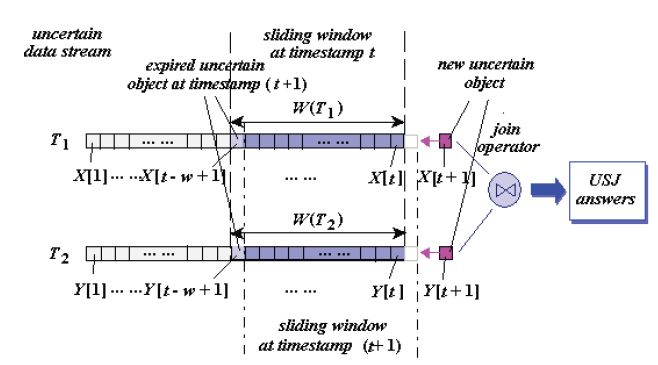
\includegraphics[scale=0.8]{figures/dataconnection.png}
	\centering
	\caption{Παράδειγμα ένταξης εικόνας από άλλο άρθρο ή βιβλίο (Πηγή: \cite{[ACC+03]})}
	\label{dataconnection}
\end{figure}

Στο κείμενό σας, πρέπει να παραθέσετε άρθρα, βιβλία, ιστοσελίδες, άλλες διπλωματικές κλπ. που διαβάσατε. Παραδείγματα παραπομπών:

* από βιβλία: \cite{[RSV02]}

* από άρθρα σε περιοδικά: \cite{[ACC+03],[DRS09],[GBE+00]}

* από άρθρα σε πρακτικά επιστημονικών συνεδρίων: \cite{[JMS+08],[MHP05],[PS11]}

* από ιστοσελίδες: \cite{[Ora11]}

* από διπλωματικές ή άλλες δημοσιευμένες εργασίες: \cite{[Pap15]}


\section{<Τίτλος για σχετική θεματική περιοχή 2>}

Γράψτε το κείμενό σας...


\chapter{Τεχνικές Προβλέψης Χρονοσειρών}
\label{chap3}

\section{Εισαγωγή}
Μέσα από την εφαρμογή των κλασικών μεθόδων προβλέψεων αποσκοπούμε με χρήση των παρελθοντικών παρατηρήσεων μιας χρονοσειράς να εκτιμήσουμε τις μελλοντικές.
Η πρόβλεψη αποτελεί μια πολυβηματική διαδικασία που θα αναπτυχθεί στο παρόν κεφάλαιο και περιγράφεται από το διάγραμμα ροής του Σχήματος \ref{classicmethodology}.

\begin{figure}[t!]
  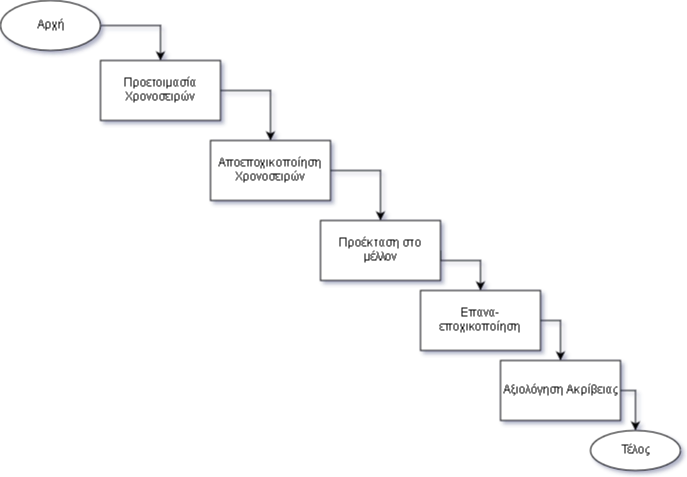
\includegraphics[scale=0.5]{figures/classicforecasting(1).png}
\centering
\caption{Κλασική μεθοδολογία πρόβλεψης χρονοσειρών}
\label{classicmethodology}
\end{figure} 



\section{Προετοιμασία Χρονοσειρών}

\subsection{Γραφική Αναπαράσταση Δεδομένων}
Κατά τη διαδικασία της επεξεργασίας και πρόβλεψης μιας χρονοσειράς είναι σημαντικό ο ερευνητής να μπορεί να αποκτήσει μία διαίσθηση πάνω στα δεδομένα. Μέσω της αναπαράστασης τους σε μια γραφική απεικόνιση μπορεί εύκολα να διαπιστώσει ποια ποιοτικά χαρακτηριστικά της χρονοσειράς έχουν έντονο βάρος. Μπορεί έτσι να εντοπίσει ότι η χρονοσειράς χαρακτηρίζεται από ακραίες τιμές, έχει έντονη τάση ή μοτίβα που επαναλαμβάνονται και εποχιακότητα.



\subsection{Διαχείριση Ιδιομορφίας Χρονοσειρών}
Είναι αρκετά σύνηθες τα δεδομένα που προορίζονται για πρόβλεψη να παρουσιάζουν δυσμορφίες. Μη σταθερή συχνότητα μεταξύ δύο συνεχόμενων τιμών μιας χρονοσειράς τη καθιστά αταίριαστη για πολλές από τις κλασικές μεθόδους πρόβλεψης. Τα δεδομένα βρίσκονται σε συχνότητα διαφορετική από αυτή που θέλουμε να προβλέψουμε, λόγου χάρη ημερήσια, ενώ είναι επιθυμητό να παραχθούν μηνιαίες προβλέψεις.
Επίσης, υπάρχει η περίπτωση ενώ εν γένει η σειρά αποτελείται από τιμές που ισαπέχουν μεταξύ τους στο πεδίο του χρόνου, παρουσιάζονται περιπτώσεις που δεν έχουν σημειωθεί κάποιες παρατηρήσεις. Αυτές τις ελλείψεις τις λέμε κενές τιμές. Μία άλλη ιδιομορφία που μπορεί να συναντήσουμε και καθιστά τη χρονοσειρά μη διαχειρίσιμη από αρκετές μεθόδους είναι η ύπαρξη μηδενικών τιμών. 

\subsubsection{Επαναδειγματοληψία}
Στη περίπτωση που το χρονικό διάστημα μεταξύ δύο παρατηρήσεων δεν είναι σταθερό ή ακόμα και διαφορετικό από αυτό που θέλουμε να έχουμε στη πρόβλεψή μας, πρέπει να φέρουμε τα δεδομένα μας σε μια πιο κανονικοποιημένη μορφή. Μία μέθοδος που μπορούμε να ακολουθήσουμε είναι η μέθοδος της επαναδειγματοληψίας (\en{resampling}). Η χρονοσειρά, συχνά, περιγράφει φαινόμενα συνεχούς χρόνου μέσα από διακριτό χρόνο. Με την επαναδειγματοληψία χρησιμοποιούμε τη πληροφορία που έχουμε ήδη στη διάθεση μας για να δημιουργήσουμε μια νέα χρονοσειρά που της έχουμε ορίσει τους ακριβείς χρόνους των παρατηρήσεων. Η επιλογή αυτή γίνεται τόσο βάσει των τιμών που ήδη έχουμε αλλά και του στόχου μας για το αποτέλεσμα στη πρόβλεψη.

Έχοντας επιλέξει τη νέα συχνότητα των δεδομένων, μένει να επιλέξουμε με ποιόν τρόπο θα γίνει η μετατροπή. Μπορούμε να διακρίνουμε δύο βασικές περιπτώσεις ανάλογα με το αν μεταβαίνουμε από μεγαλύτερη σε μικρότερη συχνότητα. Την δειγματοληψία προς τα πάνω \en{(upsampling)} και τη δειγματοληψία προς τα κάτω \en{(downsampling)}.

Για παράδειγμα, μπορούμε να έχουμε δεδομένα που έχουν συλλεχθεί σε ωριαία βάση, ενώ η πρόβλεψή μας θέλουμε να γίνει σε ημερήσιο επίπεδο. Τότε χρησιμοποιούμε \en{downsampling}, μετατρέποντας τα δεδομένα με μια κατάλληλη συνάρτηση, όπως το άθροισμα των ωριαίων τιμών, ο μέσος όρος τους, το μέγιστο ή το ελάχιστο. Αντίστοιχα αν τα δεδομένα μας θέλουμε να αλλάξουν από μικρότερη συχνότητα σε μεγαλύτερη, όπως από ημερήσια σε ωριαία, χρησιμοποιούμε \en{upsampling}, που συνδυάζεται συνήθως συμπληρώνοντας παρεμβολικά τις νέες χρονικές στιγμές που προκύπτουν. Η παρεμβολή θα περιγραφεί στη διαχείριση κενών τιμών

\subsubsection{Διαχείριση κενών τιμών}
Αρχικά, εφόσον αυτό είναι δυνατό, προσπαθούμε να βρούμε τις τιμές που μας λείπουν από άλλες πηγές, πέραν της αρχικής που λάβαμε τα δεδομένα. Επίσης, αν οι σειρές που αναλύουμε είναι λίγες στο πλήθος και γνωρίζουμε τη φύση της, μπορούμε να ορίσουμε απευθείας τις κενές τιμές, στη περίπτωση που βάσει των παραπάνω μπορούμε να κάνουμε μία ασφαλή εκτίμηση.

Στη πράξη τα παραπάνω δεν είναι συχνά εφικτά, ιδίως στις περιπτώσεις που πρέπει να γίνει διαχείριση μεγάλου αριθμού χρονοσειρών. Έτσι διακρίνουμε δύο περιπτώσεις: χρονοσειρές με εποχιακή συμπεριφορά και μη.

Όταν η χρονοσειρά προς επεξεργασία παρουσιάζει σαφή εποχιακή συμπεριφορά, μπορούμε να εκτιμήσουμε τη τιμή βάσει των τιμών των αντίστοιχων περιόδων με την εν λόγω κενή τιμή. Ένας τρόπος είναι να πάρουμε τον μέσο όρο. Έτσι, αν σε μία ετήσια χρονοσειρά με μηνιαία δεδομένα, αν μας λείπει η τιμή από κάποιον Ιανουάριο, μπορούμε να τη συμπληρώσουμε ως τον μέσο όρο των άλλων.

Στη περίπτωση που δε μιλάμε για εποχιακή συμπεριφορά, χρησιμοποιούμε τη μέθοδο της παρεμβολής για να συμπληρώσουμε τις κενές τιμές μας. Χρησιμοποιώντας τις γειτονικές τιμές μιας ακολουθίας κενών τιμών, τις συμπληρώνουμε με χρήση κατάλληλης μεθόδου. Μια κλασική προσέγγιση είναι να συμπληρωθούν γραμμικά, ως σημεία της ευθείας που ορίζουν οι δύο οριακές τιμές. Ειδάλλως μπορούμε να χρησιμοποιήσουμε άλλες μεθόδους όπως να δώσουμε τη τιμή της πιο κοντινής από τις δύο τιμές, να τις συμπληρώσουμε ως σημεία ενός πολυωνύμου δευτέρου, τρίτου ή μεγαλύτερου βαθμού. Πιο σύνθετες μέθοδοι είναι αυτές των \en{splines, krogh,} βαρυκεντρίκή και πολυωνυμική κατά σημείο.

\subsubsection{Διαχείριση μηδενικών τιμών}
Διακρίνουμε δύο περιπτώσεις, αν η παρατήρηση είναι πράγματι μηδενική ή έχει πάρει αυτή τη τιμή λόγω λάθους στη συλλογή δεδομένων. Προφανώς, στη δεύτερη περίπτωση χειριζόμαστε αυτές τιμές σαν να ήταν κενές και ακολουθούμε τις διαδικασίες που περιγράφηκαν προηγουμένως.

Αλλιώς, αν οι μηδενικές τιμές είναι λίγες, δεν θα επηρεάσουν σε μεγάλο βαθμό τα μοντέλα πρόβλεψης μας. Σε αντίθετη περίπτωση, χρησιμοποιούμε ειδικά μοντέλα για τη διαχείριση διακοπτόμενης ζήτησης.  

\subsection{Ημερολογιακές προσαρμογές}

Η χρονοσειρές είναι συχνό να περιγράφουν τιμές που σχετίζονται με ανθρώπινες ενέργειες και επηρεάζονται από τον τρόπο που είναι οργανωμένη η ανθρώπινη κοινωνία. Έτσι προετοιμάζοντας μια χρονοσειρά για πρόβλεψη πρέπει να εντοπίσουμε με πιο τρόπο συμβαίνει αυτή η επιρροή.

Σε ημερήσιες χρονοσειρές, αυτό γίνεται προσαρμόζοντας τα δεδομένα βάσει ημερολογιακών γεγονότων. Καθορίζουμε, λοιπόν, τις εργάσιμες μέρες συσχετισμένες με το μέγεθος που περιγράφει η σειρά και τις αντίστοιχες αργίες. Έχοντας προσδιορίσει τα παραπάνω, υπολογίζουμε τις εργάσιμες μέρες για κάθε περίοδο των δεδομένων μας ($N_t$) και τον μέσο όρο τους για όλες τις περιόδους ($N_{avg}$).

Μπορούμε έτσι να εξομαλύνουμε τη τιμή της κάθε παρατήρησης μας ως εξής:
\[ Y_t^{'} = Y_t . \frac{N_{avg}}{N_t} \]

\section{Προέκταση χρονοσειρών}

\subsection{Εισαγωγή}

Αφότου έχουμε προετοιμάσει τη χρονοσειρά και την έχουμε αποσυνθέσει στα επιμέρους της στοιχεία, όπως περιγράφηκε στο προηγούμενο κεφάλαιο, προχωράμε στην εφαρμογή κάποιου μοντέλου πρόβλεψης στα αποεποχικοποιημένα δεδομένα. Στόχος στην εφαρμογή του μοντέλου είναι το αποτέλεσμα που θα προκύψει να είναι όσο πιο ακριβές δύναται, δηλαδή οι τιμές που θα παράξει το μοντέλο να είναι όσο το δυνατόν πιο κοντά στις πραγματικές που θα έχουμε στη διάθεση μας με τη πάροδο του χρόνου. Στο παρόν κεφάλαιο θα μελετήσουμε τις στατιστικές μεθόδους πρόβλεψης.

\subsection{\en{Naive:} η αφελής μέθοδος}

H \en{Naive} είναι η πιο απλή μέθοδος στατιστικής πρόβλεψης. Θεωρεί ότι η τιμή που θα ακολουθήσει χρονικά ταυτίζεται με τη τιμή της παρούσας περιόδου, σύμφωνα με τη παρακάτω σχέση, όπου το $F_t$ είναι η πρόβλεψη κατά τη χρονική στιγμή $t$ και $Y_t$ η πραγματική τιμή της σειράς:
\[ F(t+1) = Y(t) \]

Είναι φυσικό ότι η \en{Naive} δεν παράγει ακριβείς προβλέψεις αλλά μπορούμε να τη χρησιμοποιήσουμε ως βάση σύγκρισης (\en{benchmark}) άλλων μεθόδων.

\subsection{Μοντέλα Παλινδρόμησης}

Η ανάλυση της παλινδρόμησης αποσκοπεί στην εύρεση συσχετίσεων μεταξύ μιας εξαρτημένης μεταβλητής και μίας ή περισσοτέρων ανεξάρτητων μεταβλητών. Έχει ευρεία χρήση στη διαδικασία των προβλέψεων, τόσο ως μοντέλο πρόβλεψης αλλά και ως υποβοήθημα σε άλλες μεθόδους, όπως θα δούμε παρακάτω. Κυρίως, όμως μας επιτρέπει να βγάλουμε συμπεράσματα για τη συσχέτιση της ανεξάρτητης μεταβλητής και των εξαρτημένων μεταβλητών.

\subsubsection{Απλή Γραμμική Παλινδρόμηση}

Η μέθοδος, που φέρει και το όνομα μέθοδος των ελαχίστων τετραγώνων, περιγράφει μία ευθεία με την ελάχιστη απόσταση ανά σημείο από τα πραγματικά δεδομένα. Για να τη λάβουμε πρέπει να ελαχιστοποιηθεί το άθροισμα σφαλμάτων στη δεύτερη εξίσωση που ακολουθεί. Επίσης, φαίνεται αναλυτικά πως προκύπτουν και οι συντελεστές:

\[\hat{Y_i} = \alpha + \beta X_i \]
\[ \sum{e_i^2} = \sum{(Y_i - \hat{Y_i})^2} \]
\[ \beta = \frac{ \frac{ \sum{X_i Y_i}}{n} - \bar{X} \bar{Y}} { \frac{\sum{X_i^2}}{n} - \bar{X}^2 } =  \frac{\sum{(X_i - \bar{X})(Y_i - \bar{Y})}} {\sum{(X_i - \bar{X})^2}} \]
\[ \alpha = \bar{Y} - \beta \bar{X} \]

Για να χρησιμοποιήσουμε τη μέθοδο της Απλής Γραμμικής Παλινδρόμησης, πρέπει να υπάρχει εξάρτηση της ανεξάρτητης μεταβλητής από τη τιμή ή τη μεταβολή κάποιας άλλης. Για να ελέγξουμε αν αυτό συμβαίνει, χρησιμοποιούμε τον συντελεστή γραμμικής συσχέτισης $r$ που αποτελεί έναν δείκτη του βαθμού που συσχετίζονται δύο μεταβλητές μεταξύ τους και για δύο μεταβλητές $X, Y$ προκύπτει ως εξής:

\[ {Cov}_{XY} = \frac{\sum{(X_i - \bar{X})(Y_i - \bar{Y})}}{n} \]
\[ {Cov}_{XX} = \frac{\sum{(X_i - \bar{X})^2}}{n} = {Var}_X = S_X^2 \]
\[ {Cov}_{YY} = \frac{\sum{(Y_i - \bar{Y})^2}}{n} = {Var}_Y = S_Y^2 \]


\[ r_{XY} = \frac{ {Cov}_{XY}} {\sqrt{{Cov}_{YY} *{Cov}_{XX} }} = \frac{ {Cov}_{XY} } { S_Y * S_X}
\]

Και προκύπτει ότι ο συντελεστής $r_{XY}$ λαμβάνει τιμές στο διάστημα από -1 έως 1.

Ο συντελεστής γραμμικής συσχέτισης επιδέχεται δύο ερμηνείες:

\begin{itemize}
    \item Μας δείχνει την κατεύθυνση της σχέσης μεταξύ των δύο μεταβλητών, δηλαδή αν όταν οι τιμές της μίας αυξάνονται, οι τιμές τις άλλης μειώνονται οι αυξάνονται. Επίσης, μπορεί να μας δείξει ότι η μεταβολές της μίας είναι ανεξάρτητες από τις άλλης.
    \item Μας δείχνει τον βαθμό συσχέτισης και συνεπώς τη δυνατότητα της γραμμής παλινδρόμησης να εκφράσει τη σχέση μεταξύ των μεταβλητών. Όσο το $r_{XY}$ πλησιάζει κατά απόλυτη τιμή τη μονάδα τόσο μικρότερη είναι η απόκλιση των πραγματικών τιμών της εξαρτημένης μεταβλητής από αυτές του μοντέλου.
\end{itemize}

Η μέθοδος των ελάχιστων τετραγώνων χρησιμοποιείται ως μοντέλο πρόβλεψης χρονοσειρών, απλά θέτοντας ως ανεξάρτητη μεταβλητή το χρόνο. Η γραμμή προκύπτει όπως περιγράψαμε προηγουμένως από τα ιστορικά δεδομένα, και προεκτείνοντας τη στο χρόνο λαμβάνουμε τις τιμές τις πρόβλεψης για τις χρονικές στιγμές που μας ενδιαφέρουν.

\subsubsection{Πολλαπλή Παλινδρόμηση}

Υπάρχουν περιπτώσεις που έχουμε πληροφορία για περισσότερες ανεξάρτητες μεταβλητές, τότε χρησιμοποιούμε τη μέθοδο της πολλαπλής παλινδρόμησης, η παίρνει την εξής μορφή:

\[ Y = \beta_0 + \beta_1 * X_1 + \beta_2 * X_2 + \dots + b_k * X_k + e \]

Αντίστοιχα με πριν, πρέπει να ελαχιστοποιηθεί το τετραγωνικό σφάλμα. Για να βρούμε τις τιμές των συντελεστών που μας οδηγούν στο ποθητό αποτέλεσμα, προσδιορίζουμε τις τιμές των μερικών παραγώγων της συνάρτησης του σφάλματος για κάθε συντελεστή. Κατόπιν λύνουμε το γραμμικό σύστημα που προκύπτει αν θέσουμε τη κάθε μερική παράγωγο ίση με το μηδέν. 




\subsection{Μοντέλα Εκθετικής Εξομάλυνσης}

Οι μέθοδοι εκθετικής εξομάλυνσης εμφανίστηκαν στο τέλος της δεκαετίας του 40', από τον \en{Brown} με σκοπό την πρόβλεψη αποθεμάτων και συνεχίζονται να εξελίσσονται ως σήμερα, αποτελώντας τις πιο δημοφιλείς μεθόδους προβλέψεων. Ο λόγος είναι ότι πρόκειται για σχετικά απλά μοντέλα με ευκολία χρήσης, μικρές υπολογιστικές απαιτήσεις και την δυνατότητα να παράξουν ακριβείς προβλέψεις ακόμα και με σχετικά μικρό ιστορικό παρατηρήσεων. Έτσι, χρησιμοποιούνται συχνά για τη παράλληλη πρόβλεψη πολλών χρονοσειρών, συνήθως με μικρό ορίζοντα πρόβλεψης. 

Σε όλα τα μοντέλα που ακολουθούν έχουμε μια εξομάλυνση των ιστορικών δεδομένων. Χρησιμοποιούνται συντελεστές βαρύτητας, που μειώνονται εκθετικά όσο πηγαίνουμε πίσω στο χρόνο, για να υπολογίσουμε τον μέσο όρο των παρατηρήσεων και να απαλλαχθούμε από τις τυχαίες διακυμάνσεις.

Προκύπτουν συνολικά 12 τύποι μοντέλων εξομάλυνσης ως συνδυασμός των παρακάτω:

\begin{itemize}
  \item Πρότυπα τάσης:

    \begin{itemize}
      \item Σταθερού Επιπέδου
      \item Γραμμικής Τάσης
      \item Εκθετικής Τάσης
      \item Φθίνουσας Τάσης
    \end{itemize}
  \item Πρότυπα εποχιακότητας:

    \begin{itemize}
      \item Άνευ Εποχιακότητας
      \item Προσθετικής Εποχιακότητας
      \item Πολλαπλασιαστικής Εποχιακότητας
    \end{itemize}
\end{itemize}

Ακολουθούν κάποια βασικά μοντέλα εκθετικής εξομάλυνσης.


\subsubsection{Απλή εκθετική εξομάλυνση}

Το μοντέλο της απλής εκθετικής εξομάλυνσης (\en{Simple Exponential Smoothing}) είναι ένα μοντέλο σταθερού επιπέδου που είναι ιδανικό για πρόβλεψη ενός βήματος. Επίσης, είναι κατάλληλο για χρονοσειρές που παρουσιάζουν υψηλό θόρυβο ή έντονο το στοιχείο της τυχαιότητας. Περιγράφεται από τις παρακάτω σχέσεις:
\[ e_t = Y_t - F_t \]
\[ S_t = S_{t-1} + \alpha * e_t \]
\[ F_{t+1} = S_t \]

Εκτός των $F_t$ και $Y_t$ που δηλώνουν τα ίδια μεγέθη όπως στη $Naive$, έχουμε το $e$ που δηλώνει το σφάλμα, το $S$ που δηλώνει το επίπεδο και το $\alpha$, τον συντελεστή εξομάλυνσης της μεθόδου με δυνατές τιμές ανάμεσα στο 0 και στο 1.
Βλέπουμε, λοιπόν, ότι πρέπει να χρησιμοποιήσουμε δύο παραμέτρους: τη πρώτη τιμή της πρόβλεψη $F_1$ και το παράγοντα εξομάλυνσης $\alpha$. Αν επιλέξουμε μεγάλη τιμή για το $\alpha$, η τελική τιμή της πρόβλεψης βασίζεται λιγότερο στις αρχικές τιμές και με $\alpha = 1$ η μέθοδος ταυτίζεται με τη \en{Naive}. Επίσης για χρονοσειρές πολύ μεγάλου μήκους η συνεισφορά της αρχικής πρόβλεψης στη τελική τιμή μειώνεται εκθετικά με το μήκος. 

Υπάρχουν διάφοροι τρόποι να ορίσουμε το αρχικό επίπεδο μια χρονοσειράς, μερικοί εκ των οποίων είναι:

\begin{itemize}
    \item Ο μέσος όρος όλων των τιμών της χρονοσειράς
    \item Ο μέσος όρος ν το πλήθος αρχικών τιμών της σειράς 
    \item Η πρώτη τιμή 
    \item Να υπολογίσουμε τη γραμμή της γραμμικής παλινδρόμησης και να θέσουμε το αρχικό επίπεδο ως το σταθερό επίπεδο αυτής της γραμμής
  \end{itemize}

Για να εντοπίσουμε τον κατάλληλο συντελεστή εξομάλυνσης για βέλτιστη ακρίβεια πρέπει να λάβουμε υπόψιν μας τόσο το θόρυβο της σειράς όσο και τη σταθερότητα του μέσου όρου της. Σε περίπτωση έντονου θορύβου, μικρή τιμή του συντελεστή μας διασφαλίζει ότι το μοντέλο μας δε θα αντιδρά υπερβολικά στο θόρυβο. Πρόσθετα, στη περίπτωση που μεταβάλλεται ο μέσος όρος των τιμών της σειράς όσο προχωράμε στο πεδίο του χρόνου, ένα μεγάλος συντελεστής εξομάλυνσης επιτρέπει στο μοντέλο να ακολουθεί αυτή τη μεταβολή. 


\subsubsection{Εκθετική εξομάλυνση γραμμικής τάσης}

Μια επέκταση της προηγούμενης μεθόδου είναι το μοντέλο εκθετικής εξομάλυνσης για γραμμικής τάση \en{Holt Exponential Smoothing} που εισήχθηκε από τον \en{Holt} το 1957. Η μέθοδος περιγράφεται από τις επόμενες εξισώσεις:

\[ e_t = Y_t - F_t \]
\[ S_t = S_{t-1} + T_{t-1} + \alpha * e_t \]
\[ T_t =  T_{t-1} + \alpha * \beta * e_t \]
\[ F_{t+m} = S_t + m * T_t \]

Όπου το νέο στοιχείο $T_t$ δηλώνει την τάση του μοντέλου κατά τη χρονική στιγμή $t$. Εδώ το $\alpha$ αποτελεί τον συντελεστή εξομάλυνσης του επιπέδου ενώ το $\beta$ το συντελεστή εξομάλυνσης της τάσης. Τόσο το αρχικό επίπεδο και η αρχική τάση πρέπει να προσδιοριστούν με προσοχή καθώς έχουν μεγάλη επιρροή στις τιμές του μοντέλου της πρόβλεψης. Για το πρώτο ακολουθούμε μία από τις μεθόδους υπολογισμού που περιγράφηκαν στην απλή εκθετική εξομάλυνση. Για την αρχική τάση μπορούμε να χρησιμοποιήσουμε μία από τις παρακάτω:

\begin{itemize}
    \item Διαφορά των δύο πρώτων τιμών της χρονοσειράς
    \item Διαφορά της τιμής μια παρατήρησης της χρονοσειράς με τη πρώτη, και διαίρεση του αποτελέσματος με τον αριθμό των χρονικών βημάτων που μεσολαβούν μεταξύ τους 
    \item Να υπολογίσουμε τη γραμμή της γραμμικής παλινδρόμησης και να θέσουμε την αρχική τάση ως τη κλίση αυτής της γραμμής
  \end{itemize}



\subsubsection{Μοντέλο μη γραμμική τάσης}

Το μοντέλο μη γραμμικής τάση εισήχθηκε το 1985 από τους \en{Gardner} και {McKenzie}, αφότου είχε παρατηρηθεί ότι το μοντέλο γραμμικής τάσης πολλές φορές παρουσίαζε θετική προκατάληψη, ειδικά όταν εφαρμοζόταν με στόχο μεσοπρόθεσμες ή μακροπρόθεσμες προβλέψεις. Το μοντέλο περιγράφεται από τις εξής σχέσεις:

\[ e_t = Y_t - F_t \]
\[ S_t = S_{t-1} + T_{t-1} + \alpha * e_t \]
\[ T_t =  T_{t-1} + \alpha * \beta * e_t \]
\[ F_{t+m} = S_t + \sum_{i=1}^{m}{\phi^{i}* T_t} \]

Παρατηρούμε ότι η αλλαγή σε σχέση με το προηγούμενο μοντέλο που περιγράψαμε εντοπίζεται στη τελευταία εξίσωση που, αντί να πολλαπλασιάζεται η τελευταία τάση που εντοπίσαμε με τη χρονική διαφορά σε περιόδους της τιμής προς πρόβλεψη από τη τελευταία τιμή των δεδομένων μας, έχουμε τη τελευταία τάση να πολλαπλασιάζεται με το άθροισμα των στοιχείων γεωμετρικής προόδου με λόγο ίσο με $\phi$ και μήκος $m$. Η παράμετρος $\phi$, που ονομάζεται παράμετρος διόρθωσης της τάσης, καθορίζει το μοντέλο ως εξής:

\begin{itemize}
\item Για $\phi = 0$, το μοντέλο ταυτίζεται με αυτό της απλής εκθετικής εξομάλυνσης
\item Για $0 < \phi < 1$, το μοντέλο χαρακτηρίζεται από φθίνουσα τάση
\item Για $\phi = 1$, το μοντέλο ταυτίζεται με το μοντέλο γραμμικής τάσης 
\item Για $\phi > 1$, έχουμε εκθετική εξομάλυνση με εκθετική τάση
\end{itemize}

Για να προσδιορίσουμε το αρχικό επίπεδο και την αρχική τάση, χρησιμοποιούμε τις μεθόδους που περιγράφηκαν στις προηγούμενες υποενότητες.


\subsection{Μέθοδος \en{Theta}}

Η μέθοδος Θ είναι μια μονοδιάστατη μέθοδος πρόβλεψης που εισήχθηκε από τον Ασημακόπουλο το 1999. Κατά το μοντέλο, η χρονοσειρά αναλύεται σε δύο ή περισσότερες χρονοσειρές ή αλλιώς γραμμές \en{Theta}. Κάθε μία από τις προκύπτουσες σειρές προβλέπεται ξεχωριστά, είτε με το ίδιο είτε με διαφορετικό μοντέλο πρόβλεψης, και η τελική πρόβλεψη είναι ο συνδυασμός των επιμέρους αποτελεσμάτων. 

Στην απλούστερη περίπτωση, το κλασσικό μοντέλο Θ, έχουμε δύο γραμμές \en{Theta}. Η πρώτη είναι μία ευθεία γραμμή που προκύπτει από την ευθεία γραμμικής παλινδρόμησης που μοντελοποιεί τα δεδομένα, η \en{Theta Line (0)}. Η δεύτερη, \en{Theta Line (2)} προκύπτει ως εξής:

\[ ThetaLine(2) = 2*Y - LRL\]

Όπου $Y$ η αρχική χρονοσειρά και $LRL$ η ευθεία που προκύπτει από τη μέθοδο ελαχίστων τετραγώνων. 

Η μέθοδος Θ βασίζεται στην μεταβολή των τοπικών καμπυλοτήτων μιας χρονοσειράς. Η μεταβολή αυτή λαμβάνει χώρα με τη χρήση της παραμέτρου θ που εφαρμόζεται στις δεύτερες διαφορές τις χρονοσειράς ως εξής: 

\[ Y_t^\theta = \theta*Y_t^{''} \]
\[ Y_t^{''} = Y_t - 2*Y_{t-1} + Y_{t-2} \]

Διακρίνουμε διαφορετικές συμπεριφορές των γραμμών Θ ανάλογα με τις τιμές τις παραμέτρου:
\begin{itemize}
    \item Αν $\theta=0$ η σειρά ταυτίζεται με την ευθεία γραμμικής παλινδρόμησης
    \item Αν $\theta=-1$ η σειρά που προκύπτει είναι η συμμετρική της αρχικής ως προς την ευθεία γραμμικής παλινδρόμησης
    \item Αν $\theta>1$ έχουμε πιο έντονες καμπυλότητες, ανάλογες του βαθμού της παραμέτρου
\end{itemize}

Το τελικό μοντέλο πρόβλεψης προκύπτει ως γραμμικός συνδυασμός των γραμμών Θ, έτσι ώστε τα βάρη της κάθε σειράς να αθροίζουν στο 1. Στην κλασσική μέθοδο, όπως είδαμε στην εξίσωση υπολογισμού της \en{Theta Line (2)}, έχουμε πάρει τα βάρη ίσα με 0.5 και για τις δύο γραμμές.

\section{Αξιολόγηση Προβλέψεων}

Αφότου έχουμε ολοκληρώσει τη διαδικασία πρόβλεψης πρέπει να αξιολογήσουμε κατά πόσο το μοντέλο μας παρήγαγε ακριβές προβλέψεις και στη περίπτωση που εφαρμόσαμε περισσότερα μοντέλα, πιο από αυτά είναι το πιο ακριβές. Για να το πετύχουμε αυτό χρησιμοποιούμε ένα σύνολο στατιστικών δεικτών αξιολόγησης της ακρίβειας. Αυτοί οι δείκτες, ή αλλιώς σφάλματα, μπορούν να χρησιμοποιηθούν για να μετρήσουν την απόδοση του υπό εφαρμογή μοντέλου στο σύνολο των δεδομένων του ιστορικού της χρονοσειράς, που είναι δηλαδή γνωστά στο μοντέλο μας (\en{in-sample error}, είναι στις τιμές του ορίζοντα πρόβλεψης (\en{out-of-sample error}). Αφότου ο σκοπός μας είναι να έχουμε ακριβή αποτύπωση της μελλοντικής εξέλιξης της χρονοσειράς, ενδιαφέρον για τη μέτρηση της απόδοσης του μοντέλου παρουσιάζει η δεύτερη κατηγορία. 

Γενικά ορίζουμε ως σφάλμα της πρόβλεψης μιας περιόδου:
\[e_i = Y_i - F_i\]

Το απλό ποσοστιαίο σφάλμα ως:
\[p_i = \frac{ 100 * e_i} { Y_i } (\%) \]

Επίσης, έχουμε το απλό σχετικό σφάλμα, που είναι ο λόγος του σφάλματος της υπό εξέταση μεθόδου σε σχέση με κάποια άλλη μέθοδο. Συνήθως η μέθοδος σύγκρισης είναι η \en{Naive}, που περιγράφηκε πρωτύτερα:

\[r_i = \frac{  e_i} { e_i^* } \]

Το απλό κανονικοποιημένο σφάλμα βρίσκεται από τη παρακάτω σχέση:

\[q_i = \frac{  e_i} { \frac{1}{n-1} \sum_{i=2}^n {|Y_i - Y_{i-1}|}} \]


Στον Πίνακα \ref{tab:errors} βλέπουμε τους πιο κοινούς δείκτες ακρίβειας. To \en{mean} υποδηλώνει τον αριθμητικό μέσο όρο, το \en{median} τη διάμεσο και το \en{gmean} το γεωμετρικό μέσο. Επίσης το \textbf{1} λαμβάνει τη τιμή 1 στη περίπτωση που αυτό που εσωκλείει είναι αληθές, αλλιώς παίρνει την τιμή 0.

\begin{table}[h]
\centering
\begin{tabular}{|c|>{\centering\arraybackslash}m{6cm}|c|}
  \hline
  \textbf{Συντομογραφία} & \textbf{Πλήρες Όνομα} & \textbf{Τύπος} \\
  \hline
  \en{ME }  &   \en{Mean Error}  & $mean(e_i)$ \\
  \en{MSE }  &   \en{Mean Squared Error}  & $mean(e_i^2)$ \\
  \en{RMSE }  &   \en{Rooted Mean Squared Error}  & $\sqrt{mean(e_i^2)}$ \\
  \en{MAE }  &   \en{Mean Absolute Error}  & $mean(|e_i|)$ \\
  \en{MdAE }  &   \en{Median Absolute Error}  & $median(|e_i|)$ \\
  \en{MAPE }  &   \en{Mean Absolute Percentage Error}  & $mean(|p_i|)$ \\
  \en{MdAPE }  &   \en{Median Absolute Percentage Error}  & $median(|p_i|)$ \\
  \en{sMAPE }  &   \en{Symmetric Mean Absolute Percentage Error}  & $mean(\frac{200*|Y_i - F_i|}{Y_i + F_i)})$ \\
  \en{sMdAPE }  &   \en{Symmetric Median Absolute Percentage Error}  & $median(\frac{200*|Y_i - F_i|}{Y_i + F_i)})$ \\
  \en{MRAE }  &   \en{Mean Relative Absolute Error}  & $mean(|r_i|)$ \\
  \en{MdRAE }  &   \en{Median Relative Absolute Error}  & $median(|r_i|)$ \\
  \en{GMRAE }  &   \en{Geometric Mean Relative Absolute Error}  & $gmean(|r_i|)$ \\
  \en{RelMAE }  &   \en{Relative Mean Absolute Error}  & $MAE/MAE_b$ \\
  \en{RelRMSE }  &   \en{Relative Mean Squared Error}  & $RMSE/RMSE_b$ \\
  \en{LMR }  &   \en{Log Mean Squared Error Ratio}  & $\log(RelMSE)$ \\
  \en{PB }  &   \en{Percentage Better}  & $100 * mean( \textbf{1}\{|r_i|<1\})$ \\
  \en{PB(MAE) }  &   \en{Percentage Better (MAE)}  & $100 * mean( \textbf{1}\{MAE<MAE_b\})$ \\
  \en{PB(MSE) }  &   \en{Percentage Better (MSE)}  & $100 * mean( \textbf{1}\{MSE<MSE_b\})$ \\
  \en{MAsE }  &   \en{Mean Absolute Scaled Error}  & $mean(|q_i|)$ \\
  \en{MdAsE }  &   \en{Median Absolute Scaled Error}  & $median(|q_i|)$ \\
  \hline
\end{tabular}
\caption{Δείκτες Ακρίβειας}
\label{tab:errors}
\end{table}


Στηριζόμενοι στη δουλειά των \en{Hyndman} και \en{Koehler} μπορούμε να χωρίσουμε τους δείκτες αυτούς στις εξής κατηγορίες:

\subsubsection{Δείκτες που εξαρτώνται από τη κλίμακα των δεδομένων}

Η κατηγορία αυτή αποτελείται από τους δείκτες \en{MSE, RMSE, MAE, MdAE} που συναρτώνται της απόλυτης τιμής των δεδομένων. Βοηθούν ιδιαίτερα όταν καλούμαστε να συγκρίνουμε την απόδοση διαφόρων μοντέλων πρόβλεψης επί της ίδιας χρονοσειράς. Σε περίπτωση που τους εφαρμόζουμε, όμως, σε ένα σύνολο χρονοσειρών με διαφορετική κλίμακα μπορούν να παράξουν αποπροσανατολιστικά αποτελέσματα. Το προτέρημα του δείκτη \en{RMSE} έναντι του απλού \en{MSE} είναι ότι μας δίνει μετρήσεις στην ίδια κλίμακα με αυτή της χρονοσειράς στην οποία εφαρμόζεται. Επίσης, οι δύο παραπάνω δείκτες είναι ιδιαίτερα ευαίσθητοι στις ακραίες τιμές μιας χρονοσειράς, σε σύγκριση με του \en{MAE, MdAE} λόγω του τετραγωνισμού του σφάλματος. Αυτό τους καθιστά ακατάλληλους για χρήση στην αξιολόγηση της ακρίβειας πρόβλεψης.

\subsubsection{Δείκτες που βασίζονται σε ποσοστιαία σφάλματα}

Σε αυτή την ομάδα, από τους δείκτες που είδαμε, ανήκουν οι \en{ MAPE, MdAPE, sMAPE} και \en{sMdAPE}. Οι δείκτες \en{MAPE} και \en{MdAPE} υστερούν στο γεγονός ότι δεν δύνανται να λάβουν τιμή όταν οι πραγματικές παρατηρήσεις είναι μηδενικές και επιπρόσθετα παρουσιάζουν έντονη ασυμμετρία όταν οι παρατηρήσεις είναι κοντά στο μηδέν. Έτσι, ο δείκτες \en{MAPE} παρουσιάζει χαρακτηριστικά μεγάλες τιμές σε σχέση με τον δείκτη \en{MdAPE}.  Μπορούμε, βέβαια, με τη χρήση λογαριθμικών μετασχηματισμών να προσδώσουμε μια σταθερότητα στους δείκτες. Επίσης, οι δύο αυτοί δείκτες δίνουν μεγαλύτερη βαρύτητα στα θετικά έναντι των αρνητικών σφαλμάτων. Αντίθετα, οι δείκτες \en{sMape} και \en{sMdAPE} δεν παρουσιάζουν στον ίδιο βαθμό το πρόβλημα των μηδενικών τιμών. Αν και το όνομα τους υποδηλώνει συμμετρία, έχουν το μειονέκτημα ότι οι αισιόδοξες και οι απαισιόδοξες προβλέψεις δεν υπολογίζονται με το ίδιο βάρος.

\subsubsection{Δείκτες σχετικών σφαλμάτων}

Από τους δείκτες που έχουμε εξετάσει οι \en{MRAE, MdRAE} και \en{GMRAE} ανήκουν σε αυτή την κατηγορία. Το πρόβλημα με αυτή των ομάδα δεικτών είναι ότι στις περιπτώσεις που το σφάλμα αναφοράς λαμβάνει αρκετά μικρές τιμές ο λόγος $r_i$ τείνει να έχει άπειρη διακύμανση.

\subsubsection{Σχετικοί δείκτες}

Το πλεονέκτημα των σχετικών δεικτών \en{RelMAE, RelRMSE} και \en{PB} είναι ότι αποφεύγουν το πρόβλημα που είδαμε στη προηγούμενη κατηγορία δεικτών με τις άπειρες τιμές. Επίσης, μας επιτρέπουν να αποφασίσουμε εύκολα πιο από τις μεθόδους που συγκρίνουμε είναι πιο ακριβής, ανάλογα με τον αν ο δείκτες έχει τιμή μεγαλύτερη της μονάδας. Βέβαια, καθότι απαιτούν αρκετές προβλέψεις δε μπορούμε να τους εφαρμόσουμε όταν έχουν πρόβλεψη με ορίζοντα ίσο με ένα. 

\subsubsection{Κανονικοποιημένοι δείκτες}

Οι κανονικοποιημένοι δείκτες \en{MAsE, MdAsE} προσφέρουν τόσο ευκολία στην ερμηνεία αντίστοιχη των σχετικών δεικτών, ενώ συγχρόνως μπορούν να εφαρμοστούν για μοναδική περίοδο πρόβλεψης. Επιπρόσθετα, είναι απαλλαγμένες από το επίπεδο της κάθε χρονοσειράς και εφαρμόσιμες σε μαζική πρόβλεψη χρονοσειρών, αποφεύγοντας τις απροσδιοριστίες των ποσοστιαίων σφαλμάτων.






\chapter{Προτεινόμενη Μεθοδολογία}
\label{chap4}

\section{Εισαγωγή}

Στις προηγούμενες παραγράφους είδαμε τη συνηθισμένη διαδικασία πρόβλεψης μιας χρονοσειράς:

\begin{enumerate}
\item Προετοιμάζουμε τα δεδομένα και τα φέρνουμε στην επιθυμητή μορφή για ανάλυση
\item Αποσυνθέτουμε τη χρονοσειρά στα επιμέρους συνθετικά της στοιχεία
\item Προεκτείνουμε με τις μεθόδου πρόβλεψης την αποεποχικοποιημένη χρονοσειρά στο μέλλον
\item Ενσωματώνουμε την εποχιακότητα στο μοντέλο πρόβλεψης
\item Αξιολογούμε την ακρίβεια της πρόβλεψης
\end{enumerate}

Μπορούμε όμως να παρατηρήσουμε ένα πρόβλημα στην παρακάτω διαδικασία. Στις περιπτώσεις που η χρονοσειρά μας δεν διαθέτει αρκετά ιστορικά δεδομένα, δεν είναι δυνατό για εμάς να εξάγουμε το στοιχείο της εποχιακότητας. Έτσι, διαχειριζόμαστε τη χρονοσειρά ως μη εποχιακή και εφαρμόζουμε τις μεθόδους πρόβλεψης στα αρχικά δεδομένα.  Είναι προφανές, όμως, ότι μπορούμε να έχουμε στη διάθεση μας χρονοσειρές που είναι εποχιακές και που θα μπορούσαμε να τις προβλέψουμε καλύτερα στη περίπτωση που είχαμε γνώση για την εποχιακή τους συμπεριφορά. 

Στη παρούσα διπλωματική προσπαθούμε να ξεπεράσουμε αυτό το πρόβλημα με χρήση της επιπλέον πληροφορίας που μπορούμε να λάβουμε από άλλες συναφείς χρονοσειρές με την υπό εξέταση χρονοσειρά. Έτσι, αν έχουμε στη διάθεσή μας δεδομένα που περιγράφουν παρόμοια μεγέθη, όπως λόγου χάρη πωλήσεις συναφών προϊόντων, υποθέτουμε ότι μπορούμε να εκμαιεύσουμε την ζητούμενη πληροφορία από το σύνολο των χρονοσειρών και να βελτιώσουμε την ακρίβεια της πρόβλεψης στις χρονοσειρές που στερούνται επαρκούς ιστορικού. 

\begin{figure}[t!]
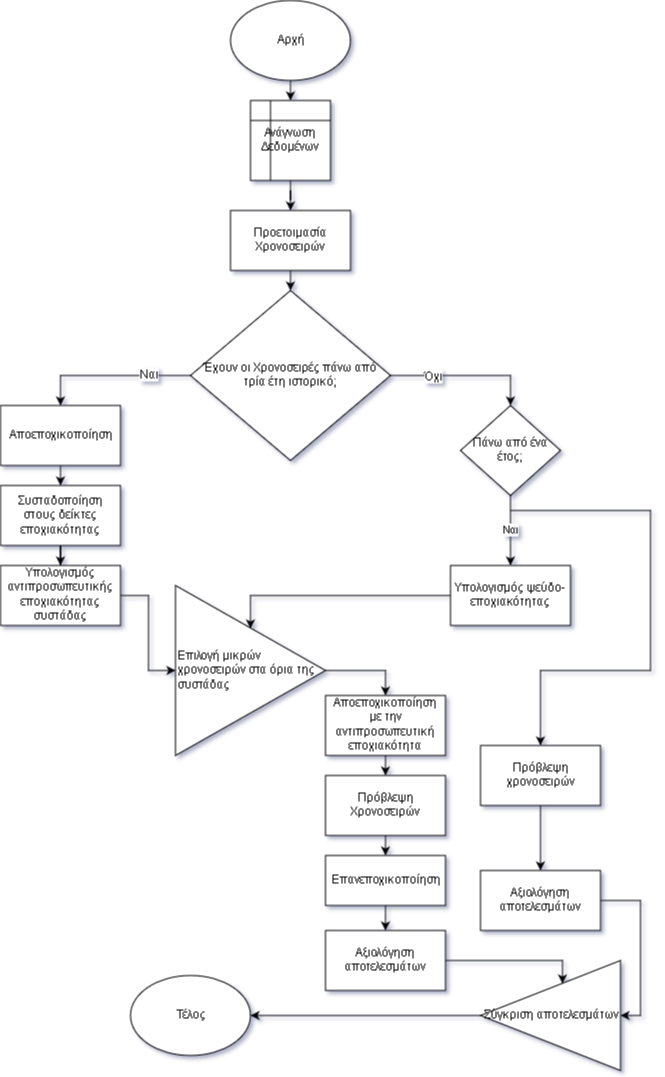
\includegraphics[scale=0.5]{figures/methodology.png}
\centering
\caption{Διάγραμμα Ροής Μεθοδολογίας}
\label{MethodologyFC}
\end{figure} 

Σε αυτό το κεφάλαιο θα περιγράψουμε πώς εξετάστηκε αυτή η υπόθεση. Αρχικά, φέρνουμε τα δεδομένα μας σε κατάλληλη μορφή για την στατιστικές μεθόδους που θέλουμε να εφαρμόσουμε. Έπειτα, χωρίζουμε τις χρονοσειρές σε δύο ομάδες: εκείνες με επαρκές ιστορικό για να εξάγουμε το στοιχείο της εποχιακότητας και τις υπόλοιπες. Στη πρώτη κατηγορία, εντοπίζουμε τους δείκτες εποχιακότητας κάθε χρονοσειρά και κατόπιν εξετάζουμε αν υπάρχει συνάφεια μεταξύ τους. Το αποτέλεσμα είναι να δημιουργηθούν συστάδες με παρόμοια εποχιακότητα και υπολογίζουμε τους αντιπροσωπευτικούς δείκτες εποχιακότητας της συστάδας. Στις χρονοσειρές που στερούνται επαρκής πληροφορίας, προσπαθούμε να βρούμε μία ψεύδο-εποχιακότητα που θα χρησιμοποιήσουμε σαν κριτήριο συνάφειας με τις συστάδες που προέκυψαν προηγουμένως. Για τις μικρές χρονοσειρές που βρέθηκε να παρουσιάζουν παρόμοια εποχιακή συμπεριφορά με κάποια ομάδα, εφαρμόζουμε τα μοντέλα πρόβλεψης κάνοντας αποεποχικοποίηση με του λόγους εποχιακότητας της συστάδας. Κατόπιν κάνουμε πρόβλεψη στις ίδιες χρονοσειρές χωρίς αποεποχικοποίηση. Τελικώς, συγκρίνουμε τα αποτελέσματα των δύο προσεγγίσεων. 

Μια αναπαράσταση της διαδικασία μπορούμε να δούμε στο διάγραμμα ροής του σχήματος \ref{MethodologyFC}.

\section{Προετοιμασία και Αποσύνθεση Χρονοσειρών}

\subsubsection{Έλεγχος τιμών, \en{resampling} και διαχείριση κενών τιμών}
Αρχικά, πρέπει να φέρουμε τα δεδομένα σε μία μορφή κατάλληλη για την ανάλυση και εφαρμογή μεθόδων που θέλουμε να κάνουμε. Για να το πετύχουμε αυτό εφαρμόζουμε τις τεχνικές επαναδειγματοληψίας και διαχείρισης κενών τιμών που αναπτύξαμε στο προηγούμενο κεφάλαιο, αφότου έχουμε επιλέξει από το σύνολο δεδομένων μας τη πληροφορία που μας είναι χρήσιμη. 

Βέβαια, η παραπάνω διαδικασία δεν μπορεί να γίνει μόνο ως κλειστό κουτί (\en{black box}, δηλαδή να διαχειρίζεται πλήρως από το σύστημά μας. Πρέπει να αποκτήσουμε μία εποπτική διαίσθηση πάνω στα δεδομένα και στηριζόμενοι στη γνώση που έχουμε για τη φύση τους να διορθώσουμε τυχούσες ατέλειες. Μία συχνή τέτοια περίπτωση είναι οι αρνητικές τιμές σε ένα φυσικό μέγεθος που δεν δύναται να παίρνει τέτοιες. 

Με παρόμοιο τρόπο πρέπει να σχεδιάσουμε τη διαδικασία του \en{resampling} και της διαχείρισης κενών τιμών. Ο λόγος είναι ότι καλούμαστε να επιλέξουμε τη κατάλληλη συνάρτηση ή προσέγγιση για να γίνουν τα παραπάνω και για να μην αλλοιωθεί η πληροφορία που φέρουν τα δεδομένα κατά αυτή τη διαδικασία, πρέπει να ορίσουμε ένα σύνολο φυσικών κανόνων που απορρέει από το προσδιορισμό της φύσης τους.

Τελικά, για να μπορέσουμε να αξιολογήσουμε τη προτεινόμενη μέθοδο πρέπει να αποκρύψουμε τις τελευταίες τιμές των χρονοσειρών μας. Το χρονικό διάστημα που αφαιρούμε από τα δεδομένα θα αποτελέσει και τον ορίζοντα πρόβλεψης των μοντέλων που θα χρησιμοποιήσουμε. Έτσι, το αποτέλεσμα των μεθόδων θα συγκριθεί με τις κρυμμένες τιμές και θα έχουμε τη δυνατότητα να αξιολογήσουμε την ακρίβεια της προσέγγισής μας.

\subsection{Αποεποχικοποίηση}

Οι μέθοδοι αποεποχικοποίησης που συναντήσαμε στο Κεφάλαιο 2, απαιτούν η αρχική μας χρονοσειρά να έχει επαρκές πλήθος δεδομένων. Κάνουμε μια διαμέριση, λοιπόν, των δεδομένων μας σε δύο ομάδες: αυτές που έχουν πάνω από τρία έτη παρατηρήσεων και αυτές που δεν έχουν. 

Ικανοποιούνται τα κριτήρια για την αποσύνθεση στη πρώτη ομάδα χρονοσειρών και εφαρμόζουμε το πολλαπλασιαστικό μοντέλο της κλασσικής μεθόδου αποσύνθεσης. Το γεγονός ότι σκοπεύουμε να χρησιμοποιούμε τους δείκτες εποχιακότητας που θα προκύψουν ως το σημείο αναφοράς για να εντοπίσουμε τις συστάδες που υπάρχουν στο σύνολο των δεδομένων μας, καθιστά την διασφάλιση της υψηλής ακρίβειας ακόμα πιο σημαντική κατά τον υπολογισμό τους. Έτσι, χρησιμοποιούμε τη μέθοδο συρρίκνωσης \en{James-Stein} κατά τη διαδικασία υπολογισμού των λόγων εποχιακότητας. Επίσης, είναι απαραίτητο όλες οι χρονοσειρές να έχουν τους δείκτες τους στην ίδια κλίμακα και συνεπώς κανονικοποιούνται έτσι ώστε το άθροισμά τους να είναι ίδιο με το μήκος της εποχιακότητας.

Πρέπει, όμως, να μπορέσουμε να αποκτήσουμε και μια εικόνα για την εποχιακότητα των χρονοσειρών που στερούνται επαρκές πλήθος παρατηρήσεων. Έτσι, για τις υπόλοιπες χρονοσειρές, θα χρησιμοποιήσουμε τους εξής τύπους για να λάβουμε το σύνολο των ``ψεύδο-εποχιακών'' δεικτών:

\[ CxSxR = \frac{Y}{LRL} \]

Θέτουμε την τάση της χρονοσειράς να είναι ίση με την ευθεία γραμμικής παλινδρόμησης επί των δεδομένων. Θεωρώντας ότι η χρονοσειρά μας είναι πολλαπλασιαστική, αφαιρούμε την τάση από τα αρχικά δεδομένα διαιρώντας την αρχική χρονοσειρά με την ευθεία ελαχίστων τετραγώνων.

\[ PS_t = mean(CxSxR_t, CxSxR+{t+l_{season}}, \dots, CxSxR_{t+i*l_{season}}), \]
\[ t+i*l_{season} < L, i=1,2,\dots \] 
\[ PS_{norm} = \frac{ PS * l_{season}}{\sum{PS_t}} \]

Όπου, PS είναι η σειρά της ψευδο-εποχιακότητας, $l_{season}$ το μήκος της εποχιακότητας και $L$ το μήκος της χρονοσειράς. Συνεπώς, ορίζουμε την ψευδο-εποχιακότητα ως το μέσο όρων των τιμών ανά περίοδο της χρονοσειράς, αφότου της έχουμε αφαιρέσει την τάση. Κατόπιν, κανονικοποιούμε το προηγούμενο αποτέλεσμα έτσι ώστε το άθροισμα των δεικτών ψευδο-εποχιακότητας να αθροίζει στο μήκος του εποχιακού μοτίβου. 

\section{Συσταδοποίηση Δεικτών Εποχιακότητας}

Έχοντας το σύνολο των εποχιακών δεικτών μπορούμε πλέον να εφαρμόσουμε ανάλυση συστάδων \en{(cluster analysis)} σε αυτό. Μας ενδιαφέρει το σύνολο των χρονοσειρών των οποίων η εποχιακότητα προέκυψε με τις κλασικές μεθόδους αποσύνθεσης. 

Για να το καταφέρουμε αυτό, θα χρησιμοποιήσουμε μεθόδους συσταδοποίησης (\en{clustering}) από το πεδίο της Μηχανικής Μάθησης (\en{Machine Learning}). Δύο μέθοδοι που ελέγξαμε είναι οι μέθοδοι \en{k-means} και \en{DBSCAN}. 

\subsection{\en{K-means}}

Ο αλγόριθμος \en{K-means} γνωστός και ως ο αλγόριθμος του \en{Lloyd}, παράγει οικογένειες δεδομένων που χαρακτηρίζονται από παρόμοια διακύμανση, προσπαθώντας να ελαχιστοποιήσει την ενδοοικογενειακό τετραγωνική διαφορά. Το πλήθος των συστάδων που θα προκύψουν από την εφαρμογή του αλγορίθμου είναι μία παράμετρος που ορίζει ο χρήστης.

Κάθε συστάδα (\en{cluster}) χαρακτηρίζεται από το κέντρο της (\en{centroid}), που ουσιαστικά είναι ο μέσος όρος όλων των στοιχείων που την αποτελούν. Βάσει αυτού, υπολογίζεται το κριτήριο της τετραγωνικής διαφοράς μια συστάδας, που προσπαθεί ο αλγόριθμος να ελαχιστοποιήσει.

Η μέθοδος χαρακτηρίζεται από τρία βασικά βήματα, που μετά το πρώτο ο αλγόριθμος επαναλαμβάνει τα άλλα δύο:

\begin{enumerate}
    \item Επιλογή αρχικών κεντρών για τις συστάδες
    \item Κατανομή των στοιχείων (εδώ χρονοσειρών) σε συστάδες, ανάλογα με την απόσταση από το κέντρο τους
    \item Υπολογισμός νέου κέντρου κάθε συστάδας, ως ο μέσος όρος των στοιχείων που την αποτελούν
\end{enumerate}

Ο αλγόριθμος σταματάει, όταν δεν έχουμε μεγάλη διαφορά μεταξύ των κεντρών που υπολογίστηκαν ανάμεσα από δύο επαναλήψεις. 

\subsection{\en{DBSCAN}}

Ο αλγόριθμος \en{DBSCAN (Density-Based Spatial Clustering of Applications with Noise)} αντιμετωπίζει τις συστάδες ως περιοχές που χαρακτηρίζονται από μεγάλη πυκνότητα και χωρίζονται μεταξύ τους από περιοχές που δεν έχουν αυτό το χαρακτηριστικό. Έτσι, σε αντίθεση με τον \en{K-means} μπορεί να παράξει συστάδες που δεν χρειάζεται να είναι σε κυρτές περιοχές του χώρου.

Στον αλγόριθμο \en{DBSCAN} δεν χρειάζεται να οριστεί από πριν το πλήθος των συστάδων, ενώ αντιμετωπίζει κάποια στοιχεία του συνόλου ως ακραίες τιμές που δεν κατατάσσει σε καμία συστάδα. Όμως, πρέπει να οριστεί τι εννοούμε πυκνή περιοχή και αυτό γίνεται με δύο παραμέτρους. Ένα βασικό στοιχείο της μεθόδου είναι τα βασικά δείγματα \en{core samples}, δηλαδή ένα δείγμα από το σύνολο των δεδομένων μας που έχει τουλάχιστον \textit{ν} το πλήθος άλλα στοιχεία του συνόλου, το πολύ σε απόσταση \textit{ε} από αυτό. Τα \textit{ν} και \textit{ε} είναι οι παράμετροι που ορίζουν πόσο πυκνό πρέπει να είναι ένα \en{cluster}.

\subsection{Επιλογή και εφαρμογή μεθόδου}

Ζητούμενο σε αυτό το βήμα της μεθοδολογίας είναι να ελέγξουμε αν πράγματι υπάρχει συνάφεια στην εποχιακή συμπεριφορά των χρονοσειρών που έχουμε στη διάθεσή μας και να κάνουμε συστάδες βάσει αυτού. Συνεπώς, η ανάλυση συστάδων γίνεται με χρήση του αλγορίθμου \en{DBSCAN}. 

Εντοπίζουμε με πειραματισμό τις κατάλληλες παραμέτρους για τον αλγόριθμο. Κριτήριο μας είναι τα \en{cluster} που προκύπτουν να μην έχουν μικρό αριθμό, έτσι ώστε να μπορεί να παραχθεί αντιπροσωπευτική εποχιακότητα μέσα από αυτό.

Έχοντας παράξει τα \en{clusters} με εφαρμογή του αλγορίθμου, πρέπει να δούμε αν οι υπόλοιπες χρονοσειρές βάσει των ψευδο-εποχιακών δεικτών, θα μπορούσαν να ανήκουν σε αυτά. Ένας τρόπος για να το διαπιστώσουμε αυτό είναι να το ελέγξουμε βάσει του κριτηρίου των τετραγώνων του \en{K-means}. Έτσι, ελέγχουμε ποια είναι η μέγιστη τετραγωνική απόσταση μέσα σε κάθε συστάδα από το κέντρο της. Αν η απόσταση της ψευδο-εποχιακότητας μιας χρονοσειράς έχει μικρότερη απόσταση από το κέντρο της συστάδας από αυτή που υπολογίσαμε, τότε την κατατάσσουμε σε αυτή. 

Τελικώς προκύπτει ένα υποσύνολο των χρονοσειρών που δεν είχαν αρκετές παρατηρήσεις να προσεγγίζουν την εποχιακή συμπεριφορά άλλων που είχαν. Έτσι μπορούμε να περιμένουμε ότι πράγματι είναι εποχιακές χρονοσειρές και χρησιμοποιώντας το κέντρο της συστάδας που την κατατάξαμε, να την αποεποχικοποιήσουμε. Μένει να δούμε αν προβλέποντας κατά αυτό τον τρόπο αποεποχικοποιημένη χρονοσειρά μπορούμε να έχουμε καλύτερα αποτελέσματα από το να κρίναμε αυτές τις χρονοσειρές μη εποχιακές και να τις προεκτείναμε ως τέτοιες.

\section{Πρόβλεψη}

Για την πρόβλεψη, τόσο των αποεποχικοποιημένων χρονοσειρών όσο και των αρχικών τους δεδομένων θα χρησιμοποιήσουμε τις μεθόδους που είδαμε στο Υποκεφάλαιο 3.3. Συγκεκριμένα θα χρησιμοποιήσουμε τις εξής μεθόδους:

\begin{itemize}
  \item \en{Naive}
  \item Γραμμική Παλινδρόμηση (\en{LRL})
  \item Απλή Εκθετική Εξομάλυνση (\en{SES})
  \item Εκθετική Εξομάλυνση Γραμμικής Τάσης (\en{Holt Exponential Smoothing})
  \item Εκθετική Εξομάλυνση Φθίνουσας Τάσης (\en{Damped Exponential Smoothing})
  \item Κλασική Μέθοδο Θ (\en{Theta Classic})
\end{itemize}

Για να βρεθούν οι βέλτιστες τιμές των παραμέτρων για κάθε μία από τις μεθόδου που εφαρμόζουμε εδώ, χρησιμοποιήθηκε το μέσο τετραγωνικό σφάλμα \en{MSE}. Συγκεκριμένα, ελέχθησαν όλες οι δυνατές τιμές των παραμέτρων με βήμα 0.01 και εκείνες που παρήγαγαν το μικρότερο μέσο τετραγωνικό εντός-του-δείγματος σφάλμα (\en{out-of-sample error}) χρησιμοποιήθηκαν για την επέκταση της χρονοσειράς στο μέλλον. 

Οι παραπάνω μέθοδοι εφαρμόστηκαν δύο φορές. Μία αφότου αποεποχικοποιήσαμε τα δεδομένα και μία στην αρχική τους μορφή. Στη πρώτη περίπτωση ενσωματώθηκε στο μοντέλο της πρόβλεψης και η εποχιακότητα της συστάδας στην οποία άνηκε η εκάστοτε χρονοσειρά.

\section{Αξιολόγηση Πρόβλεψης}

Το σημαντικότερο βήμα της διαδικασίας, καθότι αξιολογώντας της κάθε προσέγγιση και συγκρίνοντας τα αποτελέσματα μπορούμε να αποφανθούμε αν πράγματι η λύση του προβλήματος για τις μικρές εποχιακές χρονοσειρές, που προτείνεται στη παρούσα διπλωματική, προσφέρει βελτίωση στην ακρίβεια.

Στο πρόβλημα αυτό εφαρμόζουμε τον δείκτη ακριβείας σε ένα μεγάλο πλήθος χρονοσειρών που μπορεί να χαρακτηρίζεται από διαφορετικά επίπεδα στις χρονοσειρές που εμπεριέχει. Γι' αυτό τον λόγο χρειαζόμαστε ένα σφάλμα που είναι στην ίδια κλίμακα για όλες τις χρονοσειρές και παράγει διαφορετικά αποτελέσματα ανάλογα με το μέγεθος των παρατηρήσεων.

Επίσης, η χρονοσειρές, λόγω και της εποχιακότητας που τις χαρακτηρίζει, θα έχουν τιμές σε κάποιες χρονικές περιόδους που είναι πιθανό να βρίσκονται πολύ κοντά στο μηδέν. Ο δείκτης που θα χρησιμοποιήσουμε, λοιπόν, δε πρέπει να είναι ευαίσθητος στις μικρές τιμές.

Ένας δείκτης που μπορούμε να ορίσουμε που ικανοποιεί τα προαναφερθέντα κριτήρια είναι ο κανονικοποιημένος δείκτης μέσο απόλυτου σφάλματος που δίνεται από τον ακόλουθο τύπο:

\[ MAE_{norm} = mean(e_i)/mean(Y) \]

Βάσει, λοιπόν, αυτού του δείκτη βλέπουμε αν η μέθοδος μας παράγει καλύτερα αποτελέσματα ανά μέθοδο. Αυτό μπορούμε να το δούμε τόσο στο κατά μέσο όρο σφάλμα ανά μέθοδο όσο και στο ποσοστό των χρονοσειρών που παρουσίασαν πιο ακριβείς προβλέψεις με τη προτεινόμενη προσέγγιση. 

Χρησιμοποιώντας τη πληροφορία που λάβαμε από το τελευταίο βήμα, μπορούμε να δούμε πώς θα μπορούσαμε να βελτιώσουμε τη μεθοδολογία εν συνόλω.



\chapter{< τίτλος που αφορά την επίλυση του προβλήματος >, π.χ.: Επεξεργασία πιθανοτικών ερωτημάτων \tl{\textit{k}}-εγγύτερων γειτόνων}
\label{chap5}

\section{Εισαγωγή}

Εδώ εξηγούμε ότι θα περιγράψουμε το κύριο κομμάτι της διπλωματικής μας, που είναι στην ουσία η ανάπτυξη μεθόδων και αλγορίθμων για την επίλυση του προβλήματος που ορίσαμε στο προηγούμενο κεφάλαιο. 

\section{<τίτλος που αφορά τεχνική/αλγόριθμο 1, π.χ.: Εφαρμογή φίλτρων βάσει καννάβου>}

Περιγραφές μπορούν να γίνουν βάζοντας ενδεικτικά κομμάτια κώδικα ή ψευδοκώδικα, όπως ο Αλγόριθμος \ref{alg:processing} και περιγράφοντάς τα με λόγια. Μην ξεχνάτε να δίνετε πάντα παραδείγματα για το πώς τρέχει ένα κομμάτι ψευδοκώδικα π.χ. για έναν αλγόριθμο.
Αν έχετε επίσης θεωρήματα που αποδεικνύουν κάποια αποτελέσματα των τεχνικών/αλγορίθμων, τα βάζετε εδώ. 

\begin{otherlanguage}{english}
\begin{algorithm}
\caption{\ \ \ Probabilistic $k\theta NN$ Monitoring}
\begin{algorithmic}[1]
\begin{footnotesize}

\STATE{\bf Procedure} {\em VerifyCandidate} (focal query point $q$, threshold $\theta$, object $o$, list of auxiliary objects $P$, distance $kMAXDIST$) 

\IF { $\Phi(o, kMAXDIST) \geq \theta$ {\bf and} $L_2(q, o) \leq L_2(q, P.$top()) }

\STATE {$P$.pop()};   \ \ \ \ \ \ \ \ {\em //Replace the most extreme element in $P$, since candidate $o$ ... }

\STATE {$P$.push($o$)};  \ \ \ \ \ {\em //... has enough probability and has its mean closer to focal $q$ }

\ENDIF

\STATE {\bf End Procedure}


\end{footnotesize}
\end{algorithmic}
\label{alg:processing}
\end{algorithm}
\end{otherlanguage}


\section{<τίτλος που αφορά τεχνική/αλγόριθμο 2, π.χ.: Βελτιστοποίηση αναζητήσεων>}

...



%\chapter{Πειραματική Αξιολόγηση}
\label{chap6}

Στο κεφάλαιο αυτό εξηγούμε ότι θα παρουσιαστεί η πειραματική αξιολόγηση και ο έλεγχος σωστής λειτουργίας του αλγορίθμου. 


\section{Παράμετροι αξιολόγησης}

Εδώ περιγράφουμε λεπτομερώς τί παραμέτρους θα μετρήσουμε και εξηγούμε γιατί διαλέξαμε τις παραμέτρους αυτές. 

\section{Σύστημα αξιολόγησης}

Εδώ περιγράφουμε το σύστημα που χρησιμοποιήσαμε για να αξιολογήσουμε τις τεχνικές μας. Συνήθως, η περιγραφή γίνεται με κείμενο και με ένα block diagram περιγραφής των λειτουργιών του συστήματος.
Αν το σύστημα είναι μεγάλο, τότε συζητήστε με τον επιβλέποντα μήπως χρειάζεται να υπάρχει ξεχωριστό κεφάλαιο με τίτλο ` Σχεδίαση συστήματος '. 

\section{Οργάνωση πειραμάτων}

Εδώ περιγράφουμε λεπτομερώς πώς οργανώσαμε τα πειράματα. Π.χ.
α) τί σύνολο δεδομένων χρησιμοποιήσαμε (συνθετικά, έτοιμες συλλογές)
β) τί τιμές είχαν διάφοροι παράμετροι του συστήματός αξιολόγησης, κ.λ.π.

Οι τιμές των παραμέτρων μπορούν να φαίνονται και σε πίνακα, όπως λ.χ. στον Πίνακα \ref{tab:parameters}:

\begin{table}[h]
\centering
\begin{tabular}{|c|>{\centering\arraybackslash}m{8cm}|}
\hline Πλήθος κελιών καννάβου \textit{\tl{c}} $\times$ \textit{\tl{c}} & 50 $\times$ 50, 100 $\times$ 100, 200 $\times$ 200, \textbf{250} $\times$ \textbf{250}, 500 $\times$ 500, 1000 $\times$ 1000  \\
\hline Τυπική απόκλιση $\sigma$ & 25\tl{m}, 50\tl{m}, 75\tl{m}, \textbf{100\tl{m}}, 150\tl{m}, 200\tl{m} \\
\hline Αριθμός εγγύτερων γειτόνων \textit{\tl{k}} & 1, 2, \textbf{3}, 4, 5, 10, 20 \\
\hline Πιθανοτικό κατώφλι $\theta$ & 50$\%$, 60$\%$, 70$\%$, \textbf{75$\%$}, 80$\%$, 90$\%$, 99$\%$ \\
\hline  
\end{tabular}
\caption{Παράμετροι πειραμάτων}
\label{tab:parameters}
\end{table}

Αν χρησιμοποιήσατε συνθετικά δεδομένα, τότε εξηγήστε στην παρακάτω χωριστή υποενότητα τον τρόπο που τα δημιουργήσατε:

\subsection{Παραγωγή συνθετικών δεδομένων}

Τα πειραματικά δεδομένα παρήχθησαν ...


\section{Αποτελέσματα της μελέτης}

Εδώ παρουσιάζουμε τα αποτελέσματα των μετρήσεων με μορφή γραφικών παραστάσεων, όπως ενδεικτικά στο Σχ. \ref{GridGranularity}. Δίνουμε λεπτομερή εξήγηση και σχολιασμό των αποτελεσμάτων, πάντα σε σχέση με το πρόβλημα που οι τεχνικές μας φιλοδοξούν να λύσουν. 
Φροντίστε να ομαδοποιήσετε τα αποτελέσματα (σε χωριστές υποενότητες)ανάλογα με τις παραμέτρους που μετράτε, π.χ. χωριστά το κόστος σε χρόνο από το κόστος σε χώρο ή όσον αφορά την ακρίβεια των απαντήσεων.

\begin{figure}[t!]
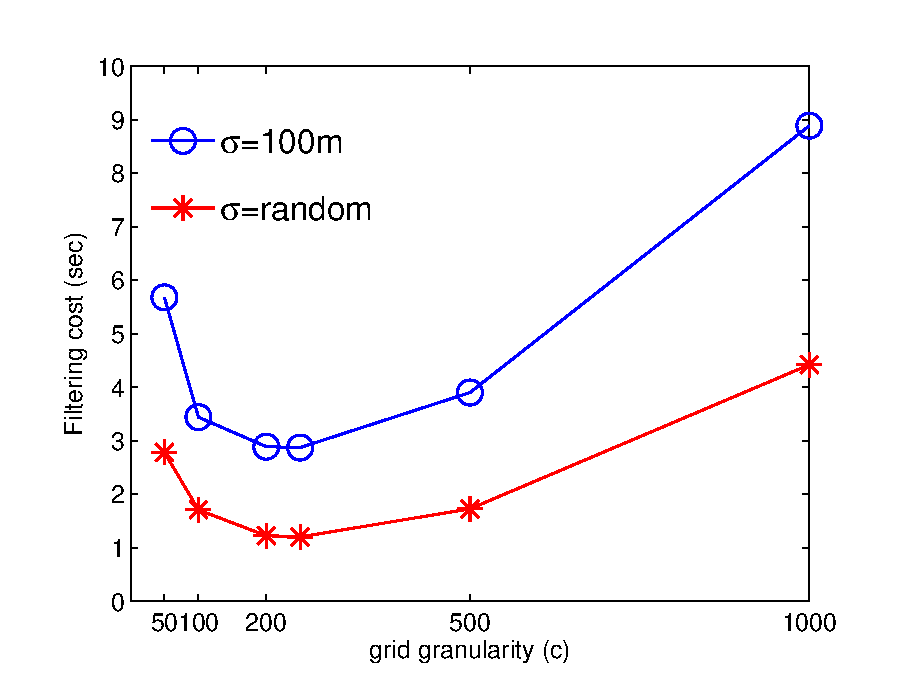
\includegraphics[scale=0.5]{figures/grid_granularity.eps}
\centering
\caption{Κλιμάκωση χρόνου εκτέλεσης για διάφορες υποδιαιρέσεις του καννάβου}	
\label{GridGranularity}
\end{figure} 


\section{Σύνοψη συμπερασμάτων αξιολόγησης}

Εδώ συνοψίζουμε τα συμπεράσματα της αξιολόγησης. Η σύνοψη να γίνεται σύντομα και καθαρά, π.χ. 1. αυτό, 2. το άλλο, κ.ο.κ.


%\chapter{Τεχνικές λεπτομέρειες}
\label{chap7}

Εδώ λέμε ότι θα ακολουθήσουν τεχνικές λεπτομέρειες της διπλωματικής.

\section{Λεπτομέρειες υλοποίησης}

Εδώ περιγράφουμε λεπτομερώς θέματα της διπλωματικής που έχουν τεχνικό ενδιαφέρον. Προσδιορίστε επομένως τα θέματα αυτά, βάλτε μια ενότητα για κάθε ένα και περιγράψτε τα αναλυτικά. Η περιγραφή μπορεί να γίνει βάζοντας κομμάτια κώδικα ή ψευδοκώδικα, και περιγράφοντάς τα με λόγια. Μην ξεχνάτε να δίνετε πάντα παραδείγματα για το πώς τρέχει ένα κομμάτι κώδικα π.χ. για έναν αλγόριθμο.

\subsection{<Τίτλος θέματος 1>}
Γράψτε το κείμενό σας εδώ ...

\subsection{<Τίτλος θέματος 1>}
Γράψτε το κείμενό σας εδώ ...

\section{Πλατφόρμες και προγραμματιστικά εργαλεία}

Εδώ περιγράφονται τα χαρακτηριστικά της συγκεκριμένης υλοποίησης, όπως η πλατφόρμα ανάπτυξης και εκτέλεσης, τα προγραμματιστικά εργαλεία, οι απαιτήσεις της εφαρμογής σε hardware, κ.λ.π. Επίσης, περιγράφεται λεπτομερώς η διαδικασία εγκατάστασης της διπλωματικής σε υπολογιστή. Προσέξτε να δίνονται όλες οι λεπτομέρειες, το απαραίτητο λογισμικό και οι αναγκαίες ρυθμίσεις.

\chapter{Επίλογος}
\label{chap8}

Σε αυτό το κεφάλαιο θα σκιαγραφήσουμε την πορεία ανάλυσης των δεδομένων που μας οδήγησαν εν τέλει στη διαδικασία της πρόβλεψης και επικύρωσης της υπόθεσής μας. Θα συζητήσουμε τα αποτελέσματα που προέκυψαν και τι περαιτέρω βήματα μπορούν να γίνουν για να ισχυροποιήσουν αυτά τα αποτελέσματα. 

\section{Σύνοψη και συμπεράσματα}

Στις κλασική μεθοδολογία πρόβλεψης μιας χρονοσειράς, αφού την προετοιμάσουμε την αποσυνθέτουμε στα βασικά της χαρακτηριστικά: τη τάση, τον κύκλο, την τυχαιότητα και την εποχιακότητα. Αφότου έχουμε υπολογίσει τους εποχιακούς δείκτες, τους χρησιμοποιήσουμε για να απαλλάξουμε τα αρχικά δεδομένα από τις αλλαγές που υφίστανται λόγω της περιόδου που βρίσκονται μέσα στο μήκος του μοτίβου της εποχιακότητας. Έτσι προκύπτει μία πιο σταθερή πλέον χρονοσειρά, αφού της έχουμε αφαιρέσει τις προβλεπόμενες διακυμάνσεις. Αυτή τη χρονοσειρά, λοιπόν, χρησιμοποιούμε ως είσοδο στο μοντέλο της πρόβλεψής μας. Κατόπιν, λαμβάνουμε το αποτέλεσμα του μοντέλου και ενσωματώνουμε την εποχιακή συμπεριφορά για να προκύψει η τελική πρόβλεψη. 

Το πρόβλημα εμφανίζεται όταν η υπό εξέταση χρονοσειρά δεν χαρακτηρίζεται από επαρκώς μεγάλο ιστορικό για να μας επιτρέψει να εξάγουμε το μοτίβο της εποχιακότητάς της. Σε αυτή τη περίπτωση, η συνηθισμένη προσέγγιση είναι να αντιμετωπίζουμε τη χρονοσειρά ως μη εποχιακή και να τη προβλέπουμε χωρίς να κάνουμε ανάλυση εποχιακότητας. Όμως, οι εποχιακές διακυμάνσεις, σε περίπτωση που η σειρά περιέγραφε πράγματι ένα εποχιακό μέγεθος, συνεχίζουν να χαρακτηρίζουν τα δεδομένα και τελικώς επηρεάζουν την ακρίβεια των μοντέλων.

Παράλληλα, όσο περνάνε τα χρόνια το πλήθος των δεδομένων που εν γένει έχουμε στη διάθεσή μας αυξάνεται εκθετικά. Αυτό το γεγονός ανοίγει δρόμους σε νέες προσεγγίσεις για να προσπαθήσουμε να αυξήσουμε την ακρίβεια της διαδικασίας της πρόβλεψης. Έτσι, θεωρώντας ότι έχουμε ένα μεγάλο πλήθος χρονοσειρών που περιγράφουν παρόμοιας φύσης δεδομένα, υποθέσαμε ότι μπορούμε να εκμαιεύσουμε πληροφορία για την εποχιακή συμπεριφορά των δεδομένων της συγκεκριμένης φύσης.

Δοκιμάσαμε την υπόθεσή μας σε ένα σύνολο δεδομένων χρονοσειρών από τα δεδομένα για τον όγκο υγρού φυσικού αερίου σε δεξαμενές. Στόχος ήταν να μπορέσουμε να εκτιμήσουμε σε ποια χρονική στιγμή στο μέλλον κάθε δεξαμενή θα αδειάσει με σκοπό να το αποτρέψουμε, έτσι ώστε να μην υπάρξει πρόβλημα στους πελάτες της εταιρίας που παρέχει το φυσικό αέριο αλλά και να της δώσουμε τη γνώση που χρειάζεται για να σχεδιάσει βέλτιστα τον ανεφοδιασμό των δεξαμενών.

Πρώτο βήμα στην ανάλυση ήταν να καθαρίσουμε τα δεδομένα μας και να τα φέρουμε στη μορφή που θα μας βοηθήσει να πετύχουμε τον στόχο μας. Φροντίσαμε, λοιπόν, να τα φέρουμε όλα σε ημερήσια συχνότητα και να διαχειριστούμε τις κενές και μηδενικές τιμές. Κατόπιν, είδαμε ότι για να προβλέψουμε πότε θα καταναλωθεί όλο το υγρό φυσικό αέριο στις δεξαμενές μας ενδιαφέρει ο ρυθμός κατανάλωσης σε κάθε μία από αυτές. Έτσι, παίρνοντας τις διαφορές μεταξύ δύο διαδοχικών ημερών στον όγκο του υγρού, λάβαμε την ημερήσια κατανάλωση. Σκοπεύοντας να προβλέψουμε μεσοπρόθεσμα το πότε θα αδειάσει μία δεξαμενή, υπολογίσαμε τον μέσο όρο της ημερήσια κατανάλωσης για κάθε μήνα και προέκυψε η μηνιαία χρονοσειρά της μέσης κατανάλωσης. 

Τελειώνοντας, λοιπόν, το πρώτο βήμα της ανάλυσης καταλήξαμε να έχουμε ένα σύνολο χρονοσειρών που περιγράφουν την μέση μηνιαία κατανάλωση ανά δεξαμενή. Όλες αυτές η χρονοσειρές μετράνε παρόμοια μεγέθη, ενώ ανάμεσά τους υπάρχει ένα ποσοστό που δεν έχουν επαρκή δεδομένα για να εξάγουμε την εποχιακή τους συμπεριφορά. Από την άλλη, η κατανάλωση φυσικού αερίου, που είναι συνδεδεμένη άμεσα με την θερμοκρασία αφότου μία κύρια χρήση του είναι η θέρμανση, περιμένουμε να χαρακτηρίζεται από εποχιακές διακυμάνσεις στο μήκος του χρόνου. 

Έτσι, διαμερίσαμε τις χρονοσειρές σε αυτές που μπορούμε να χρησιμοποιήσουμε τις κλασικές μεθόδους αποσύνθεσης και σε αυτές που δεν μπορούμε. Στη πρώτη κατηγορία τις εφαρμόσαμε κανονικά και λάβαμε τους δώδεκα ετήσιους δείκτες εποχιακότητας για κάθε μία εξ' αυτών. Για τη δεύτερη κατηγορία αφαιρέσαμε από την χρονοσειρά τις τιμές της ευθείας γραμμικής παλινδρόμησης που αντιστοιχούσαν σε κάθε παρατήρηση, και από το αποτέλεσμα πήραμε τον μέσο όρο των τιμών για κάθε περίοδο. Προέκυψαν, συνεπώς, δώδεκα τιμές που ονομάσαμε δείκτες ψευδο-εποχιακότητας.

Επόμενο βήμα ήταν να ελέγξουμε αν πράγματι υπήρχαν κοινά μοτίβα στην εποχιακότητα των χρονοσειρών της πρώτης κατηγορία και να τα εντοπίσουμε. Για αυτό το λόγο χρησιμοποιήσαμε τον αλγόριθμο συσταδοποίησης \en{DBSCAN}. Βρήκαμε, ότι αν και πολλές χρονοσειρές δεν ακολουθούσαν συγκεκριμένο μοτίβο, υπήρχε ένα σύνολο εξ αυτών που παρουσίαζε συνάφεια στους εποχιακούς του δείκτες. Γι' αυτό το μοτίβο υπολογίσαμε την μέση εποχιακότητα.

Για να ελέγξουμε αν οι χρονοσειρές με μικρό ιστορικό ανήκουν στην συστάδα που προέκυψε, χρησιμοποιήσαμε το κριτήριο με το οποίο ο αλγόριθμος \en{k-means} κατατάσσει τα δεδομένα που πραγματεύεται σε συστάδες. Έτσι, για το σύνολο των χρονοσειρών με συνάφεια στους δείκτες εποχιακότητας, υπολογίσαμε τη μέγιστη μέση τετραγωνική διαφορά του κέντρου από τους δείκτες των υπόλοιπων του χρονοσειρών. Αν η μέση τετραγωνική διαφορά μεταξύ των δεικτών ψευδο-εποχιακότητας και του κέντρου ήταν μικρότερη από το αποτέλεσμα, θεωρήσαμε ότι μπορεί να αντιπροσωπευθεί η εποχιακότητα των χρονοσειρών τους από αυτή του κέντρου.

Έχοντας στη διάθεση μας ένα σύνολο χρονοσειρών που πληρούσε πλήρως τα κριτήρια που θέσαμε για την υπόθεσή μας περάσαμε στη διαδικασία της πρόβλεψης. Αρχικά, προβλέψαμε τις χρονοσειρές κατά την κλασική προσέγγιση: τις προεκτείναμε στο μέλλον βάσει των αρχικών τους δεδομένων. Έπειτα, αποεποχικοποιήσαμε αυτές τις χρονοσειρές, με τους μέσους δείκτες εποχιακότητας της συστάδας, και εφαρμόσαμε τα μοντέλα πρόβλεψης κατόπιν. Στη δεύτερη περίπτωση, πολλαπλασιάσαμε πάλι τους δείκτες εποχιακότητας με το προϊόν των μοντέλων.

Σε ποσοστό μεγαλύτερο του 70\% για κάθε μέθοδο πρόβλεψης είχαμε η προτεινόμενη μέθοδος να έχει μεγαλύτερη ακρίβεια, σημειώνοντας χαμηλότερη τιμή σφάλματος σε κάθε μία από τις μεθόδους που εξετάσαμε. Το αποτέλεσμα αυτό επαλήθευσε την υπόθεσή μας και έδειξε τη σημασία της διαχείρισης της εποχιακότητας των χρονοσειρών ακόμα και όταν αυτές έχουν μικρό ιστορικό.

Από τις μεθόδους που χρησιμοποιήσαμε μεγαλύτερη βελτίωση είδαμε στην ακρίβεια της μεθόδου της γραμμικής παλινδρόμησης. Παράλληλα, είχαμε το μεγαλύτερο ποσοστό των χρονοσειρών που πήγε καλύτερα η προτεινόμενη μέθοδος.  Αυτό είναι λογικό, καθότι η μέθοδος υπολογίζει την τάση της χρονοσειράς και την προεκτείνει στο μέλλον. Δεδομένου ότι οι υπό εξέταση χρονοσειρές έχουν μικρό ιστορικό ενώ χαρακτηρίζονται από εποχιακή συμπεριφορά, η γραμμή ελαχίστων τετραγώνων επηρεάζεται από τις κορυφές τις χρονοσειράς και τις βλέπει σαν αύξηση της τάσης. 

Τόσο η προτεινόμενη όσο και η κλασική προσέγγιση είχαν μεγαλύτερη ακρίβεια για τη μέθοδο \en{Naive}. Αυτό συμβαίνει διότι σε τόσο μικρό αριθμό δεδομένων η επιρροή της τυχαιότητας είναι πολύ μεγάλη κατά την πρόβλεψη.

\section{Μελλοντικές επεκτάσεις}

Στη παρούσα εργασία είδαμε ότι εκμεταλλευόμενοι την πληροφορία που μας δίνεται από έναν μεγάλο όγκο συναφών δεδομένων μπορούμε να εκτιμήσουμε την εποχιακή συμπεριφορά μικρότερων χρονοσειρών εξ αυτών.

Βέβαια, η μελέτη έγινε σε ένα συγκεκριμένο σύνολο χρονοσειρών ενεργειακών χρονοσειρών. Το πρώτο βήμα, λοιπόν, είναι να εξεταστούν και άλλα σύνολα δεδομένων. Ιδιαίτερο ενδιαφέρον, δε, θα έχει η μελέτη οικονομικών δεδομένων και η εφαρμογή στη διαχείριση αποθήκης.

Ένας άλλος παράγοντας που αξίζει να εξεταστεί είναι εναλλακτικές μέθοδοι αποσύνθεσης της χρονοσειράς. Αντί της κλασικής πολλαπλασιαστικής μεθόδου αποσύνθεσης, μπορεί να γίνει ανάλυση με το προσθετικό μοντέλο ή το μοντέλο \en{STL}, που είδαμε επίσης σε προηγούμενο κεφάλαιο. Επίσης, μπορεί να χρησιμοποιηθεί διαφορετική μέθοδος συρρίκνωσης συντελεστών για τους δείκτες εποχιακότητας, ενώ θα μπορούσε να εφαρμοστεί συρρίκνωση και στους δείκτες ψευδο-εποχιακότητας.

Όσον αναφορά την ανάλυση συστάδων, εκτός των \en{DBSCAN} και \en{k-means} θα μπορούσαν να χρησιμοποιηθούν και άλλοι αλγόριθμοι συσταδοποίησης. Επιπρόσθετα, στη περίπτωση που το σύνολο δεδομένων περιέχει και άλλες πληροφορίες που να δίνουν μεγαλύτερη διάσταση σε αυτά, όπως λόγου χάρη τοποθεσία ή είδος πελάτη, θα μπορούσε να χρησιμοποιηθεί αυτή σαν παράμετρος στην ανάλυση συστάδων.

Μεγάλο ενδιαφέρον θα παρουσίαζε επίσης, η σύγκριση της προτεινόμενης μεθόδου με άλλες προσεγγίσεις προέκτασης χρονοσειρών. Μπορεί να γίνει σύγκριση με μεθόδους πρόβλεψης με χρήση νευρωνικών δικτύων, μοντέλων \en{ARIMA} και με μπεϋζιανές τεχνικές προβλέψεων. 



%OPTION #1: Embed bibliography from file `references.tex' using plain references.
%
\begin{thebibliography}{1}

\addcontentsline{toc}{chapter}{Βιβλιογραφία}

\bibitem{[ACC+03]} {\textlatin{
D.~J. Abadi, D.~Carney, U.~{\c{C}}etintemel, M.~Cherniack, C.~Convey, S.~Lee,  M.~Stonebraker, N.~Tatbul, and S.~Zdonik. 
Aurora: a new model and architecture for data stream management.
{\em The VLDB Journal -- The International Journal on Very Large Data Bases}, 12(2):120--139, 2003}}.

\bibitem{[DRS09]} {\textlatin{
N.~Dalvi, C.~R{\'e}, and D.~Suciu. Probabilistic databases: Diamonds in the dirt. {\em Communications of the ACM}, 52(7):86--94, July 2009}}.

\bibitem{[GBE+00]} {\textlatin{
R.~H. G{\"u}ting, M.~H. B{\"o}hlen, M.~Erwig, C.~S. Jensen, N.~A. Lorentzos,
  M.~Schneider, and M.~Vazirgiannis.
A foundation for representing and querying moving objects.
{\em ACM Transactions on Database Systems (TODS)}, 25(1):1--42, 2000}}.

\bibitem{[JMS+08]} {\textlatin{
N.~Jain, S.~Mishra, A.~Srinivasan, J.~Gehrke, J.~Widom, H.~Balakrishnan,
  U.~{\c{C}}etintemel, M.~Cherniack, R.~Tibbetts, and S.~Zdonik.
Towards a streaming {SQL} standard.
In {\em Proceedings of the VLDB Endowment}, 1(2):1379--1390, 2008}}.

\bibitem{[MHP05]} {\textlatin{
K.~Mouratidis, D.~Papadias, and M.~Hadjieleftheriou. 
Conceptual partitioning: an efficient method for continuous nearest
  neighbor monitoring.
In {\em Proceedings of the 24th ACM SIGMOD International
  Conference on Management of Data}, pages 634--645, 2005}}.

\bibitem{[Ora11]} {\textlatin{
{Oracle, Inc}.
Complex event processing {CQL} language reference.
\url{http://docs.oracle.com/cd/E16764_01/doc.1111/e12048/intro.htm }
  2009. Last accessed on 15/09/2013}}.

\bibitem{[PS11]} {\textlatin{
K.~Patroumpas and T.~Sellis.
Subsuming multiple sliding windows for shared stream computation.
In {\em Advances in
  Databases and Information Systems}, volume 6909 of Springer {\em Lecture Notes in
  Computer Science}, pages 56--69, 2011}}.

\bibitem{[RSV02]} {\textlatin{
P.~Rigaux, M.~Scholl, and A.~Voisard.
{\em Spatial databases: with application to {GIS}}.
Morgan Kaufmann, 2001}}.

\bibitem{[Pap15]}
Σεραφείμ Παπαδιάς.
Απόρριψη φόρτου από ρεύματα
  τροχιάς κινούμενων αντικειμένων. Διπλωματική Εργασία {\textlatin{\em DIPL-2015-02}} στο
Εργαστήριο Συστημάτων Βάσεων Γνώσεων και Δεδομένων, Εθνικό Μετσόβιο
  Πολυτεχνείο, Ιούλιος 2015.

\end{thebibliography}
%\addcontentsline{toc}{chapter}{Βιβλιογραφία}

%OPTION #2: Alternatively, prepare properly formatted BibTeX entries in file `references.bib'. 
%After processing with BibTeX, a file `main.bbl' is automatically populated and it is actually used for producing references in the resulting pdf. 
%IMPORTANT: You must manually modify `main.bbl' by adding \selectlanguage{english} (TOP) and \selectlanguage{english} (BOTTOM) in order to correctly display Latin and Greek characters in the final text.
\nocite{*}
\bibliography{references}


\appendix
\chapter{Τεχνικές λεπτομέρειες}
\label{chap7}

Εδώ λέμε ότι θα ακολουθήσουν τεχνικές λεπτομέρειες της διπλωματικής.

\section{Λεπτομέρειες υλοποίησης}

Εδώ περιγράφουμε λεπτομερώς θέματα της διπλωματικής που έχουν τεχνικό ενδιαφέρον. Προσδιορίστε επομένως τα θέματα αυτά, βάλτε μια ενότητα για κάθε ένα και περιγράψτε τα αναλυτικά. Η περιγραφή μπορεί να γίνει βάζοντας κομμάτια κώδικα ή ψευδοκώδικα, και περιγράφοντάς τα με λόγια. Μην ξεχνάτε να δίνετε πάντα παραδείγματα για το πώς τρέχει ένα κομμάτι κώδικα π.χ. για έναν αλγόριθμο.

\subsection{<Τίτλος θέματος 1>}
Γράψτε το κείμενό σας εδώ ...

\subsection{<Τίτλος θέματος 1>}
Γράψτε το κείμενό σας εδώ ...

\section{Πλατφόρμες και προγραμματιστικά εργαλεία}

Εδώ περιγράφονται τα χαρακτηριστικά της συγκεκριμένης υλοποίησης, όπως η πλατφόρμα ανάπτυξης και εκτέλεσης, τα προγραμματιστικά εργαλεία, οι απαιτήσεις της εφαρμογής σε hardware, κ.λ.π. Επίσης, περιγράφεται λεπτομερώς η διαδικασία εγκατάστασης της διπλωματικής σε υπολογιστή. Προσέξτε να δίνονται όλες οι λεπτομέρειες, το απαραίτητο λογισμικό και οι αναγκαίες ρυθμίσεις.

\chapter{Αναλυτικά Αποτελέσματα}

Ακολουθούν τα αναλυτικά αποτελέσματα ακρίβειας των μεθόδων με τη προτεινόμενη μέθοδο στις αριστερές στήλες και την κλασική στις δεξιές:

\begin{longtable}{|r|rrrrrr|rrrrrr|}


 \hline
  &   \en{DES} &   \en{HES} &   \en{LRL} &  \en{Naive} &  \en{SES} & Θ &   \en{DES} &   \en{HES} &   \en{LRL} &  \en{Naive} &  \en{SES} &  Θ  \\ 
 \hline
1 & 1.46 & 1.66 & 1.45 & 1.39 & 1.39 & 1.53 & 1.99 & 2.25 & 3.15 & 1.8 & 1.84 & 2.05 \\ 
2 & 0.9 & 0.99 & 0.99 & 1.0 & 0.84 & 0.82 & 1.04 & 1.06 & 1.06 & 1.0 & 1.0 & 1.03 \\ 
3 & 0.97 & 0.93 & 0.93 & 0.85 & 1.11 & 1.07 & 1.04 & 1.37 & 2.25 & 1.37 & 1.37 & 1.37 \\ 
4 & 0.86 & 0.83 & 0.94 & 0.85 & 0.85 & 0.84 & 0.87 & 1.06 & 3.64 & 1.01 & 1.01 & 1.04 \\ 
5 & 0.7 & 0.67 & 0.67 & 0.86 & 0.75 & 0.75 & 1.19 & 1.19 & 1.24 & 1.13 & 1.19 & 1.19 \\ 
6 & 0.77 & 0.76 & 1.38 & 0.73 & 0.78 & 0.77 & 0.99 & 1.04 & 5.62 & 1.04 & 1.04 & 1.04 \\ 
7 & 0.66 & 0.77 & 0.77 & 0.67 & 0.35 & 0.44 & 1.1 & 1.08 & 1.08 & 0.78 & 1.16 & 1.12 \\ 
8 & 0.67 & 0.65 & 0.54 & 0.69 & 0.67 & 0.66 & 0.6 & 0.76 & 1.01 & 0.87 & 0.87 & 0.82 \\ 
9 & 0.5 & 0.47 & 0.46 & 0.5 & 0.5 & 0.48 & 0.46 & 0.51 & 0.72 & 0.51 & 0.51 & 0.51 \\ 
10 & 0.33 & 0.35 & 0.35 & 0.82 & 0.71 & 0.3 & 1.32 & 1.43 & 1.31 & 1.44 & 1.44 & 1.44 \\ 
11 & 10.52 & 4.28 & 4.28 & 1.0 & 18.86 & 14.15 & 1.0 & 3.7 & 30.34 & 1.0 & 11.37 & 6.76 \\ 
12 & 1.04 & 0.9 & 0.87 & 1.29 & 1.29 & 1.09 & 0.98 & 0.75 & 1.54 & 1.05 & 1.05 & 0.8 \\ 
13 & 2.98 & 2.6 & 2.6 & 1.21 & 3.79 & 3.75 & 0.97 & 0.97 & 3.22 & 1.23 & 1.23 & 0.97 \\ 
14 & 3.4 & 4.72 & 4.29 & 5.02 & 5.02 & 4.87 & 0.74 & 5.79 & 15.39 & 6.63 & 6.63 & 6.21 \\ 
15 & 0.81 & 0.74 & 0.7 & 0.87 & 0.82 & 0.78 & 0.56 & 0.57 & 0.57 & 0.83 & 0.55 & 0.55 \\ 
16 & 0.89 & 0.89 & 0.74 & 0.91 & 0.88 & 0.89 & 0.85 & 1.36 & 1.77 & 1.39 & 1.41 & 1.39 \\ 
17 & 1.0 & 1.0 & 0.65 & 0.99 & 0.99 & 1.0 & 1.0 & 1.0 & 3.18 & 1.0 & 1.0 & 1.0 \\ 
18 & 0.76 & 0.69 & 0.69 & 0.83 & 0.91 & 0.92 & 1.29 & 1.3 & 2.07 & 1.17 & 1.29 & 1.29 \\ 
19 & 0.5 & 0.5 & 0.55 & 0.5 & 0.5 & 0.5 & 0.83 & 0.94 & 1.27 & 0.43 & 0.43 & 0.43 \\ 
20 & 0.6 & 0.59 & 0.59 & 0.6 & 0.61 & 0.6 & 0.56 & 0.39 & 0.75 & 0.33 & 0.33 & 0.36 \\ 
21 & 1.51 & 1.49 & 1.22 & 1.51 & 1.51 & 1.5 & 1.67 & 1.77 & 2.46 & 1.79 & 1.79 & 1.78 \\ 
22 & 0.41 & 0.4 & 0.4 & 0.43 & 0.43 & 0.42 & 0.5 & 0.44 & 0.91 & 0.43 & 0.43 & 0.43 \\ 
23 & 0.46 & 0.5 & 0.64 & 0.46 & 0.46 & 0.47 & 0.25 & 0.33 & 2.33 & 0.26 & 0.26 & 0.29 \\ 
24 & 0.85 & 0.86 & 0.89 & 0.83 & 0.83 & 0.85 & 0.9 & 0.9 & 0.9 & 0.89 & 0.89 & 0.9 \\ 
25 & 0.5 & 0.51 & 0.56 & 0.53 & 0.53 & 0.52 & 1.35 & 1.71 & 3.77 & 1.72 & 1.72 & 1.71 \\ 
26 & 0.62 & 0.61 & 0.64 & 0.62 & 0.62 & 0.62 & 0.75 & 0.46 & 1.36 & 0.48 & 0.48 & 0.47 \\ 
27 & 0.44 & 0.43 & 0.43 & 0.74 & 0.63 & 0.53 & 1.0 & 1.04 & 3.08 & 0.95 & 1.04 & 1.04 \\ 
28 & 0.62 & 0.7 & 0.87 & 0.63 & 0.63 & 0.67 & 0.93 & 1.0 & 2.81 & 0.78 & 0.78 & 0.78 \\ 
29 & 0.76 & 0.71 & 0.71 & 0.71 & 0.71 & 0.71 & 1.0 & 1.0 & 1.88 & 1.1 & 1.1 & 1.1 \\ 
30 & 0.55 & 0.57 & 0.57 & 0.58 & 0.5 & 0.5 & 1.0 & 0.89 & 1.51 & 0.89 & 0.89 & 0.89 \\ 
31 & 0.73 & 0.69 & 0.69 & 0.69 & 0.8 & 0.78 & 1.04 & 1.02 & 1.3 & 1.0 & 1.0 & 1.01 \\ 
32 & 1.0 & 0.69 & 0.69 & 0.98 & 0.59 & 0.64 & 1.0 & 0.75 & 3.21 & 0.97 & 0.97 & 0.86 \\ 
33 & 0.48 & 0.45 & 0.45 & 0.42 & 0.55 & 0.53 & 0.94 & 0.75 & 1.65 & 0.78 & 0.78 & 0.76 \\ 
34 & 0.89 & 0.93 & 4.34 & 0.52 & 0.53 & 0.81 & 1.0 & 0.58 & 11.11 & 0.26 & 0.33 & 0.37 \\ 
35 & 1.0 & 1.0 & 1.15 & 1.0 & 1.0 & 1.0 & 1.0 & 0.97 & 5.45 & 1.0 & 1.0 & 0.99 \\ 
36 & 0.72 & 0.97 & 0.97 & 0.81 & 1.1 & 0.81 & 1.16 & 1.0 & 1.0 & 0.73 & 4.55 & 3.16 \\ 
37 & 0.73 & 0.76 & 0.76 & 0.58 & 0.56 & 0.64 & 1.05 & 1.11 & 2.96 & 1.12 & 1.12 & 1.11 \\ 
38 & 0.92 & 0.85 & 1.02 & 0.92 & 0.92 & 0.89 & 1.0 & 0.81 & 2.72 & 0.95 & 0.95 & 0.87 \\ 
39 & 0.56 & 0.54 & 0.54 & 0.61 & 0.63 & 0.62 & 0.74 & 0.83 & 1.38 & 0.58 & 0.73 & 0.78 \\ 
40 & 0.6 & 0.58 & 0.58 & 0.6 & 0.66 & 0.63 & 0.89 & 0.79 & 0.79 & 0.37 & 1.16 & 0.98 \\ 
41 & 0.43 & 0.39 & 0.39 & 0.42 & 0.42 & 0.41 & 0.38 & 0.41 & 0.62 & 0.41 & 0.41 & 0.41 \\ 
42 & 0.61 & 0.6 & 1.05 & 0.61 & 0.61 & 0.61 & 0.96 & 0.46 & 5.8 & 0.55 & 0.55 & 0.51 \\ 
43 & 0.62 & 0.76 & 4.62 & 0.64 & 0.64 & 0.82 & 1.09 & 1.15 & 6.07 & 1.18 & 1.18 & 1.17 \\ 
44 & 0.89 & 0.88 & 0.88 & 0.85 & 0.94 & 0.91 & 0.49 & 0.57 & 2.28 & 0.49 & 0.51 & 0.54 \\ 
45 & 0.54 & 0.61 & 1.06 & 0.96 & 0.52 & 0.57 & 1.0 & 0.51 & 5.27 & 0.96 & 0.96 & 0.72 \\ 
46 & 0.84 & 0.96 & 0.96 & 0.4 & 0.68 & 0.78 & 1.0 & 3.08 & 3.08 & 0.85 & 1.04 & 1.04 \\ 
47 & 0.51 & 0.47 & 0.47 & 0.55 & 0.54 & 0.53 & 0.37 & 0.37 & 0.82 & 0.37 & 0.37 & 0.37 \\ 
48 & 0.32 & 0.24 & 0.24 & 1.08 & 0.77 & 0.59 & 1.69 & 1.97 & 3.39 & 1.77 & 1.77 & 1.84 \\ 
49 & 0.38 & 0.41 & 0.41 & 0.29 & 0.3 & 0.33 & 1.0 & 0.99 & 1.66 & 0.85 & 0.99 & 1.0 \\ 
50 & 1.18 & 1.03 & 1.03 & 2.08 & 2.59 & 1.58 & 6.59 & 5.62 & 5.62 & 3.29 & 11.4 & 9.2 \\ 
51 & 0.9 & 0.81 & 1.16 & 0.9 & 0.9 & 0.86 & 0.94 & 0.75 & 4.36 & 0.94 & 0.94 & 0.84 \\ 
52 & 0.52 & 0.57 & 0.57 & 0.93 & 0.51 & 0.45 & 1.0 & 0.62 & 3.73 & 0.91 & 0.91 & 0.69 \\ 
53 & 0.49 & 0.4 & 0.7 & 0.5 & 0.5 & 0.45 & 1.21 & 1.26 & 1.78 & 1.26 & 1.26 & 1.26 \\ 
54 & 0.51 & 0.84 & 0.84 & 0.55 & 0.53 & 0.41 & 1.32 & 1.16 & 1.16 & 0.86 & 0.98 & 1.92 \\ 
55 & 1.0 & 1.0 & 1.0 & 1.0 & 0.59 & 0.95 & 0.96 & 1.01 & 1.01 & 1.0 & 2.07 & 1.53 \\ 
56 & 0.68 & 0.82 & 0.82 & 0.71 & 0.82 & 0.72 & 1.11 & 1.11 & 2.3 & 1.0 & 1.11 & 1.11 \\ 
57 & 1.02 & 1.0 & 1.0 & 0.9 & 0.9 & 1.01 & 1.0 & 1.01 & 2.02 & 1.11 & 1.11 & 1.04 \\ 
58 & 0.62 & 0.64 & 0.64 & 0.61 & 0.58 & 0.61 & 0.76 & 0.83 & 2.97 & 0.8 & 0.8 & 0.8 \\ 
59 & 0.69 & 0.77 & 0.77 & 0.66 & 0.91 & 0.89 & 1.35 & 1.36 & 3.68 & 1.37 & 1.37 & 1.36 \\ 
60 & 0.78 & 0.8 & 0.8 & 0.83 & 0.83 & 0.8 & 0.37 & 0.38 & 0.35 & 0.48 & 0.35 & 0.36 \\ 
61 & 1.0 & 0.99 & 0.6 & 0.99 & 0.99 & 0.99 & 1.0 & 0.99 & 3.54 & 1.0 & 1.0 & 0.99 \\ 
62 & 0.68 & 0.66 & 0.51 & 0.71 & 0.68 & 0.67 & 1.0 & 0.54 & 2.37 & 0.67 & 0.67 & 0.6 \\ 
63 & 1.0 & 0.89 & 1.0 & 0.88 & 0.88 & 0.55 & 0.94 & 0.84 & 1.56 & 1.09 & 1.09 & 0.94 \\ 
64 & 0.92 & 1.0 & 1.0 & 0.41 & 0.5 & 0.38 & 0.87 & 0.89 & 0.89 & 0.58 & 3.02 & 2.93 \\ 
65 & 0.91 & 0.78 & 0.51 & 0.74 & 0.74 & 0.76 & 1.0 & 1.0 & 3.51 & 0.8 & 0.8 & 0.7 \\ 
66 & 0.74 & 0.7 & 0.7 & 0.61 & 1.1 & 0.88 & 1.2 & 0.99 & 0.99 & 0.52 & 0.52 & 0.58 \\ 
67 & 0.73 & 0.72 & 0.72 & 0.73 & 0.73 & 0.73 & 0.9 & 0.99 & 0.66 & 0.26 & 0.26 & 0.23 \\ 
68 & 0.39 & 0.45 & 0.45 & 0.46 & 0.26 & 0.24 & 0.59 & 0.79 & 0.9 & 0.58 & 0.58 & 0.66 \\ 
69 & 1.0 & 0.8 & 1.1 & 0.92 & 0.92 & 0.86 & 1.0 & 1.08 & 5.7 & 1.1 & 1.1 & 1.09 \\ 
70 & 0.55 & 0.56 & 0.56 & 0.5 & 0.55 & 0.55 & 0.95 & 1.0 & 2.28 & 1.18 & 1.18 & 1.15 \\ 
71 & 0.61 & 0.62 & 0.62 & 0.61 & 0.61 & 0.61 & 0.85 & 0.22 & 0.97 & 0.27 & 0.27 & 0.24 \\ 
72 & 0.62 & 0.86 & 0.86 & 0.46 & 0.55 & 0.46 & 0.95 & 0.97 & 2.2 & 0.8 & 0.8 & 0.8 \\ 
73 & 0.82 & 0.68 & 0.68 & 0.48 & 1.01 & 0.95 & 1.0 & 1.08 & 2.08 & 0.83 & 0.93 & 0.96 \\ 
74 & 0.46 & 0.38 & 0.38 & 0.83 & 1.22 & 0.86 & 0.97 & 0.97 & 3.62 & 0.81 & 0.81 & 0.95 \\ 
75 & 1.69 & 1.92 & 1.92 & 0.98 & 1.1 & 1.34 & 1.29 & 2.71 & 7.19 & 1.48 & 1.48 & 2.1 \\ 
76 & 1.97 & 1.49 & 0.98 & 2.13 & 2.46 & 1.98 & 1.67 & 1.5 & 1.34 & 2.69 & 3.38 & 2.03 \\ 
77 & 0.44 & 0.45 & 0.48 & 0.36 & 0.36 & 0.41 & 0.77 & 0.82 & 2.38 & 0.84 & 0.84 & 0.83 \\ 
78 & 0.55 & 0.58 & 0.58 & 0.45 & 0.41 & 0.48 & 0.97 & 0.53 & 2.53 & 0.61 & 0.61 & 0.54 \\ 
79 & 0.62 & 0.69 & 0.69 & 0.49 & 0.49 & 0.52 & 0.64 & 0.82 & 2.76 & 0.69 & 0.69 & 0.71 \\ 
80 & 0.43 & 0.44 & 0.56 & 0.41 & 0.43 & 0.44 & 0.97 & 0.79 & 1.88 & 0.79 & 0.79 & 0.79 \\ 
81 & 0.86 & 1.0 & 1.0 & 0.71 & 0.71 & 0.99 & 1.01 & 1.0 & 1.2 & 0.92 & 0.92 & 1.04 \\ 
82 & 0.58 & 0.59 & 0.59 & 0.52 & 0.54 & 0.55 & 0.54 & 0.93 & 2.21 & 0.6 & 0.6 & 0.59 \\ 
83 & 0.49 & 0.51 & 0.51 & 0.5 & 0.5 & 0.49 & 0.54 & 0.47 & 1.39 & 0.54 & 0.54 & 0.5 \\ 
84 & 1.0 & 0.55 & 1.73 & 0.89 & 0.89 & 0.72 & 1.0 & 1.07 & 8.42 & 1.12 & 1.12 & 1.08 \\ 
85 & 0.57 & 0.61 & 0.61 & 0.89 & 0.37 & 0.41 & 1.83 & 2.05 & 3.58 & 1.83 & 1.83 & 1.94 \\ 
86 & 0.54 & 0.6 & 0.6 & 0.41 & 0.45 & 0.5 & 0.72 & 1.24 & 3.21 & 0.65 & 0.78 & 0.93 \\ 
87 & 0.68 & 0.81 & 0.81 & 0.53 & 0.53 & 0.48 & 0.33 & 0.34 & 1.15 & 0.35 & 0.35 & 0.35 \\ 
88 & 0.45 & 0.45 & 0.45 & 0.46 & 0.5 & 0.47 & 1.66 & 1.87 & 1.87 & 0.38 & 0.39 & 0.46 \\ 
89 & 0.64 & 0.81 & 1.61 & 0.54 & 0.54 & 0.67 & 1.04 & 1.0 & 6.91 & 0.78 & 0.78 & 0.87 \\ 
90 & 4.04 & 4.54 & 4.54 & 2.69 & 2.23 & 3.11 & 4.41 & 7.15 & 13.5 & 3.79 & 3.79 & 5.47 \\ 
91 & 0.87 & 0.93 & 0.93 & 0.49 & 0.49 & 0.59 & 0.56 & 0.94 & 1.64 & 0.39 & 0.39 & 0.38 \\ 
92 & 0.42 & 0.49 & 0.49 & 0.43 & 0.43 & 0.4 & 0.88 & 0.94 & 2.5 & 0.54 & 0.54 & 0.56 \\ 
93 & 0.44 & 0.48 & 0.48 & 0.81 & 0.19 & 0.25 & 1.0 & 1.0 & 2.59 & 0.75 & 0.75 & 0.46 \\ 
94 & 1.81 & 2.06 & 2.06 & 0.7 & 0.86 & 1.37 & 1.0 & 1.0 & 7.33 & 1.42 & 1.42 & 1.44 \\ 
95 & 0.97 & 0.98 & 0.85 & 0.96 & 0.96 & 0.97 & 1.0 & 0.76 & 0.74 & 0.96 & 0.96 & 0.86 \\ 
 \hline  
\caption{Δείκτες Ακρίβειας για όλες τις χρονοσειρές}
\end{longtable}




%\include{proofs}

\newcommand{\gloss}[2]{#1 \> \en{#2}\\ }

\chapter{����������� ����� ����}

\begin{tabbing}
%ta 'a' rythmizoun to platos ton dyo stilon
  aaaaaaaaaaaaaaaaaaaaaaaaaaaaaaaaaaa \= aaaa\kill
  \Large\textbf{���������} \> \Large\textbf{�������� ����} \\
  \gloss{�������}{sibling}
  \gloss{��������������}{idempotency}
  %\gloss{������������}{identifier}
  \gloss{�������� �����������}{information retrieval}
  \gloss{������������������}{commutativity}
  \gloss{��������}{descedant}
  \gloss{����������}{absorption}
  \gloss{���� ���������}{database}
  \gloss{��������}{attribute}
  \gloss{������������}{interface}
  \gloss{�������}{difference}
  \gloss{��������� ���������}{portal catalog}
  \gloss{�������� ����}{lattice}
  \gloss{������� �����������}{structural queries}
  \gloss{������� �������}{structural relationships}
  \gloss{������ �����}{schema}
  \gloss{����������}{validity}
  \gloss{�����}{union}
\end{tabbing}


\backmatter
\printindex

\end{document}
